\documentclass[a4paper,12pt]{book}
\usepackage{graphicx} % For graphics
\usepackage{hyperref} % For hyperlinks
% \usepackage{makeidx} % For making an index
\usepackage{float}
\usepackage{tikz}
\usepackage{amsmath}
\usepackage{enumitem}
\usepackage{pgfplots}
\pgfplotsset{compat=newest}

\newcommand{\inputtoc}[1]{\input{#1}}

% ... (rest of your preamble)

% \makeindex % Command to make the index

\pgfmathdeclarefunction{csc}{1}{%
  \pgfmathparse{1/sin(#1)}%
}


\newenvironment{exercise}[1][]
  {\par\medskip\noindent\textbf{Exercise #1} \rmfamily}
  {\medskip}

% \newenvironment{solution}[1][]
%   {\par\noindent\textbf{Solution #1} \rmfamily}
%   {\medskip}


% Define the problem environment
% \newcounter{problem}
% \newenvironment{problem}[1][\theproblem]
% {\refstepcounter{problem}\par\medskip\noindent\textbf{Problem~#1:} \rmfamily}{\medskip}

% Define the solution environment
% \newenvironment{solution}[1][]
% {\par\noindent\textit{Solution:} \rmfamily}{\medskip}


% Define the problem environment
\newcounter{problem}
\newenvironment{problem}[1][\theproblem]
{\refstepcounter{problem}\par\medskip\noindent\textbf{Problem~#1:} \rmfamily}{\medskip}

% Define the solution environment
\newenvironment{solution}[1][]
{\par\noindent\textit{Solution:} \rmfamily}{\medskip}





\begin{document}

% --- Book Cover ---
\begin{titlepage}
    \begin{tikzpicture}[remember picture, overlay]
        % Background color
        \fill[cyan!30] (current page.south west) rectangle (current page.north east);

        % Decorative Circles Pattern at the bottom
        \foreach \i in {0,...,36}
        {
            \fill[cyan!40, rotate around={10*\i:(current page.center)}] 
                (current page.south) circle (1cm);
        }
        
        % Title and additional info
        \node at (current page.center) [font=\Huge, text width=0.8\textwidth, align=center] 
            {\textbf{Pre-Calculus in Brief with Python, Colab, GitHub, and \LaTeX  \\ PCiB - Version 0.3}};
            
        \node[align=center, font=\large] at (current page.center) 
            [yshift=-2.5cm] {\today}; % <- This is the compilation date
            
        \node[align=center, font=\large] at (current page.center) 
            [yshift=-3.5cm] {MIT License};
        
        \node[align=center, font=\large] at (current page.center) 
            [yshift=-5cm] {Available on GitHub at: \\ 
            \url{https://GitHub.com/nicholaskarlson/PCiB}};
    \end{tikzpicture}
\end{titlepage}

% --- Table of Contents ---
\tableofcontents
\cleardoublepage

% --- Preface ---
\chapter*{Preface}
\addcontentsline{toc}{chapter}{Preface}
This text, \emph{Pre-Calculus in Brief - PCiB} aspires to be more than just another math book. This book strives to foster collaborative math writing. Note that this book has very few references. The reader is encouraged to use resources available on the Web to fact-check. This book's view on ``causation'' and facts is heavily influenced by Mosteller and Tukey \cite{mosteller1977}.

\section*{Redefining the Role of the Reader}
Pre-Calculus in Brief (PCiB) is an endeavor to reshape how math is written, understood, and studied. It's not just a passive read but an open-source approach to math, aiming to encourage students to become proactive learners.

This project strives to break the traditional mold of math education and invites readers and professional mathematicians to participate actively.

\section*{A Dynamic Relationship with Math}
\emph{Pre-Calculus in Brief} is not just a book but a movement and methodology, heralding a new era in how we approach, consume, and interact with math. By positioning the reader as an integral part of the math-book process, PCiB fosters a dynamic relationship with math, making mathematics more accessible, proactive, and relevant. In this shifting paradigm, we are all potential mathematicians, creators of interesting and relevant ways to learn and study math.

Please fork the LaTeX source code for PCiB (available on GitHub) and create your own book that chooses the facts and exercises most relevant to you! Also, starring the PCiB project on GitHub would be greatly appreciated! Thanks for reading PCiB!

% --- Chapters ---
\chapter{Introduction to PCiB}
\subsection*{Welcome to PCiB on GitHub}
Pre-Calculus in Brief, abbreviated PCiB, isn't merely a passive read. It's an endeavor to reshape how math is written, studied, and taught. By presenting an open-source approach to math, the goal is to encourage everyone to become proactive readers and writers of math. 

\subsection*{Fostering a Proactive Engagement with Math}

\emph{Pre-Calculus in Brief} is a call for a renewed engagement with mathematics. PCiB is an endeavor to reshape how math is written, understood, and studied. It's not just a passive read but an open-source approach to math, aiming to encourage students to become proactive learners.

This project strives to break the traditional mold of math education and encourages readers and professional mathematicians to participate actively.

\bigskip
\noindent
Please fork the \LaTeX{} source code for PCiB (available on GitHub) and create your own book on Pre-Calculus that chooses the content most relevant to you! Also, starring the PCiB project on GitHub would be greatly appreciated! Thanks for reading PCiB!

\chapter{Open-Source Ethos}
\section*{The Spirit of Shared Knowledge and Collaboration}
Math, like software, is better when it's open. PCiB draws inspiration from the open-source software movement; this section elucidates how a collaborative, transparent, and shared approach can enhance our understanding of math. Here, we look at the philosophy behind open-source and how it beautifully combines with the study of mathematics.

\subsection*{Open-Source Math: Preserving Tradition Through Collaborative Exploration}
Mathematics, like software, thrives when it embraces openness and transparency. PCiB takes a leaf from the proven benefits of the open-source software model; this section highlights how a collaborative and transparent method can improve and deepen our grasp of math and its texts. Here, we explore the principles of open source and how these principles align with the development of mathematics and its texts.

\subsection*{Understanding the Open-Source Ethos}
The open-source paradigm revolves around shared ownership, collaboration, and the free exchange of knowledge. In the software realm, this approach has led to groundbreaking innovations built and enhanced by a global community of skilled contributors. United by a mutual objective, these individuals pool their diverse talents and insights to improve and share software solutions for broader public benefit.

\subsection*{Advantages of the Open-Source Framework in Math}
\subsubsection*{Collective Insight}
Mirroring the collaborative essence of open-source software, many individuals can offer their perspectives and knowledge, making math texts more robust and varied.

\subsubsection*{Enhancement and Accuracy}
Open platforms foster an environment of constructive criticism, ensuring prompt identification and correction of inaccuracies. This meticulous peer review can help provide a credible and current mathematical text.

\subsubsection*{Universal Access}
Much as open-source software promotes free access and modification, open-source math prioritizes universal accessibility. This ensures mathematics knowledge isn't restricted to a select few but is available to all curious minds.

\subsection*{Potential Challenges}
Despite its advantages, melding open-source with math has potential pitfalls. The volume of contributions can complicate accuracy verification processes. 

However, the very community championing this open-source approach to math can serve as its vigilant protector. They can ensure that contributions undergo rigorous evaluation and referencing, akin to the meticulous checks within the open-source software community.

\subsection*{Conclusion: Reinvigorating Our Experience with Math}
Adopting an open-source perspective to the approach of math signifies a refreshed approach. It beckons a worldwide community to collaborate and forge a comprehensive and exciting math text. In this refreshed approach, every individual can play a part, both as a contributor and a learner. Math texts, through this lens, evolve and flourish, reflecting the collective input of active participants.

\chapter{Introduction to GitHub}
\section*{The Hub for Modern Collaboration}
\subsection*{Harnessing GitHub: A New Frontier in Collaborative Math Writing}
At the heart of our collaborative math endeavor lies GitHub, a platform traditionally associated with code but now repurposed for our endeavor. This section provides a primer on GitHub, laying the foundation for those unfamiliar and offering insights into its transformative potential for collective math writing, learning, and teaching.

\subsection*{A Brief Introduction to GitHub}
Originally conceptualized as a platform for developers, GitHub is a repository hosting service that facilitates version control using Git. At its core, it allows multiple users to work on a project simultaneously, tracking changes and ensuring that the latest version of a project is always accessible. Over the years, GitHub has grown beyond its initial software-centric confines, becoming a hub for all kinds of collaborative projects, from writing to data science and now to math.

\subsection*{Repurposing GitHub for Math Texts}
\subsubsection*{Version Control}
Math writing, like software, is dynamic and constantly evolving. As new sources or perspectives emerge, math texts may need revisions. GitHub's version control ensures that every change made to a document is tracked, enabling mathematicians to see how math texts evolve over time.

\subsubsection*{Collaborative Writing}
Multiple contributors can work on a single math text simultaneously. This multi-user capability ensures diverse viewpoints can be seamlessly integrated, making the math text richer and more comprehensive.

\subsubsection*{Review and Feedback}
Just as developers review and comment on code, mathematicians can provide feedback on written content. This feature encourages rigorous peer review, ensuring accuracy and credibility.

\subsubsection*{Open Access}
Math texts on GitHub can be made public, granting anyone access to read, contribute, or fork the text into their own versions. This workflow democratizes math texts, making the creation process a collective endeavor rather than the domain of a select few.

\subsubsection*{Transparency}
All changes and contributions are logged, providing a clear trail of the evolution of a mathematical text. This transparency bolsters the credibility of the text hosted on the platform.

\subsubsection*{Community Building}
Beyond just writing, GitHub fosters a community of mathematicians, enthusiasts, and readers who can discuss, debate, and engage in meaningful dialogues about math and available math texts on GitHub.

\subsection*{Conclusion: Envisioning a Collaborative Mathematical Landscape}
Embracing GitHub as a tool for collaborative math signifies more than just a shift in approach; it heralds a new era of inclusivity, transparency, and dynamism in writing, learning, and math teaching. 

\chapter{Encouragement to Fork}
\subsection*{Invitation to Dive Deep and Make It Your Own}
PCiB isn't a static entity. It thrives on evolution, adaptation, and diversification, much like math itself. We encourage readers to "fork" (a term soon to be discussed) and create their own versions of this book. Read this section to understand the essence of "forking" and how it can be the starting point of your unique math journey.

\subsection*{The Concept of Forking: A Brief Overview}

In the realm of software development, particularly in platforms like GitHub, "forking" refers to the act of creating a copy of a project, allowing one to make changes independently of the original. In this context, forking PCiB enables readers to take the base content and adapt, modify, and expand upon it, tailoring the narrative to resonate with their perspectives, insights, and understanding.

\subsection*{How to Begin Your Forking Journey}

Start Small: You don't need to rewrite entire chapters. Begin by adding annotations, insights, or even footnotes to existing content. As you grow more confident, you can expand and modify larger sections.

Engage with the Community: Share your forked version with other readers. This encourages discourse, debate, and constructive feedback, allowing your text to be refined and enhanced.

Celebrate input: Encourage others around you to fork and create their own versions. The more in-depth the input, the deeper our collective understanding of math potentially becomes.

\subsection*{Conclusion: The Power of Collective Math}

The invitation to fork PCiB isn't just about creating different versions of a book. It's a call to embrace collective writing, learning, and teaching. By embracing the essence of forking, math is not just something we read but something we actively shape, share, and pass on.

\chapter{More About GitHub}
\section*{Discovering the Power of Collaborative Tools}
Diving deeper into the world of GitHub, this chapter provides a comprehensive overview. Beyond its technicalities, we explore how GitHub emerged as a revolutionary platform for collaboration and how it can be leveraged for those interested in writing, teaching, and learning about math.

\subsection*{The Genesis of GitHub}
GitHub began as a platform designed for software developers to manage and track changes to their codebase. Launched in 2008, it swiftly gained traction due to its user-friendly interface and efficient version control system powered by Git. Over the years, it evolved from a mere repository hosting service to a dynamic hub of collaboration, housing millions of projects and engaging tens of millions of users worldwide.

\subsection*{GitHub: More than Just Code}
While GitHub's origins are rooted in code collaboration, its adaptable nature has made it a favored platform for various non-code projects. Writers, designers, educators, and researchers have discovered the potential of GitHub as a tool for:

\subsubsection*{Document Collaboration}
With its built-in version control, contributors can track changes, revert to previous versions, and seamlessly merge updates.

\subsubsection*{Project Management}
With features like "issues" and "milestones," teams can organize tasks, set goals, and monitor progress.

\subsubsection*{Open Access \& Transparency}
Public repositories allow for open contributions, ensuring transparency and fostering a sense of collective ownership.

\subsubsection*{Collaborative Writing}
Multiple contributors can simultaneously work on a single document, with every change being tracked and attributed, facilitating teamwork on extensive projects like books or research papers.

\subsubsection*{Engaging the Public}
With the platform's inherent transparency, researchers can make their work-in-progress accessible to the public, inviting insights, corrections, and contributions.

\subsection*{Case Study: PCiB's Use of GitHub}
PCiB's journey on GitHub is a testament to the platform's potential in mathematical endeavors. By hosting the book on GitHub, the following is possible:

\subsubsection*{Feedback Loop}
Readers can raise "issues," pointing out inaccuracies, suggesting enhancements, or even recommending new sections or topics.

\subsubsection*{Forking}
As previously discussed, readers can "fork" the repository, creating their unique versions of the book while staying connected to the original.

\subsubsection*{Regular Updates}
With math being dynamic, the book can be regularly updated, with new versions being released as and when significant changes are incorporated.

\subsection*{Challenges and Considerations}
While GitHub offers many advantages, it's essential to understand its limitations:

\subsubsection*{Learning Curve}
For those unfamiliar with Git or version control, there can be an initial learning curve.

\subsubsection*{Data Overwhelm}
With vast amounts of data and contributions, ensuring quality and accuracy can be challenging.

\subsubsection*{Diverse Audience Management}
Catering to both tech-savvy and non-tech audiences might require creating additional resources or tutorials to ensure inclusivity.

\subsection*{Conclusion: GitHub – A Paradigm Shift in Collaboration}
The rise of GitHub marks a significant shift in how we perceive and participate in collaborative projects. Its adaptability, transparency, and user-centric design make it a powerful tool, not just for coders but for anyone passionate about collective endeavors. In the realm of mathematics, GitHub promises a future where texts are continually refined, expanded, and enriched by a global community.

\chapter{Forking Process}
\section*{The Heart of Collaboration on GitHub}
The beauty of open-source lies in its democratization of content creation. In this section, we demystify the process of "forking" on GitHub, guiding you step-by-step on how to take PCiB and create a version uniquely yours.

\subsection*{Understanding Forking}
Before diving into the specifics, it's crucial to understand what "forking" means in the context of GitHub. In the simplest terms, to "fork" a project means to create a personal copy of someone else's project. Forking allows you to freely experiment with changes without affecting the original project. Forking is akin to taking a book you admire and making a copy to write your notes, edits, or additional chapters without altering the original book.

\subsection*{Why Fork?}
\subsubsection*{Experimentation}
It provides a safe space where you can test out ideas, make changes, or introduce new content.

\subsubsection*{Personalization}
For projects like PCiB, it allows readers to customize the content, tailor it to their perspectives, or even localize it for specific audiences.

\subsubsection*{Collaboration}
If you believe your changes have broad appeal, you can propose that they be incorporated back into the original project, enriching it with your unique contributions.

\subsection*{Step-by-Step Forking Guide}
\subsubsection*{Set Up Your GitHub Account}
If you don't have an account on GitHub, you'll need to create one. Visit GitHub's official site and sign up.

\subsubsection*{Navigate to the PCiB Repository}
Once logged in, search for the PCiB project or navigate to its URL directly.

\subsubsection*{Click the 'Fork' Button}
The fork button is located at the top right corner of the repository page; this button will create a copy of PCiB in your account.

\subsubsection*{Clone Your Forked Repository}
Forking allows you to have a local copy on your computer, making editing and experimentation easier. Use the command: \texttt{git clone [URL of your forked repo]}.

\subsubsection*{Make Your Changes}
Using your preferred tools, introduce the edits, additions, or modifications you desire.

\subsubsection*{Commit and Push Changes}
Once satisfied, save these changes (known as a "commit") and then "push" them to your forked repository on GitHub.

\subsubsection*{Optional – Create a Pull Request}
If you believe your changes should be incorporated into the original PCiB repository, you can create a "pull request." A pull request notifies the original authors of your suggestions.

\subsection*{Things to Keep in Mind}
\subsubsection*{Stay Updated}
The original PCiB project may undergo updates. It's a good practice to regularly "pull" from the original repo to keep your fork up-to-date.

\subsubsection*{Engage with the Community}
Open-source thrives on community interactions. Engage in discussions, seek feedback, and please remain open to constructive criticism.

\subsection*{Conclusion: Embracing the Forking Culture}
Forking is more than just a technical process; it symbolizes the ethos of open-source — a world where knowledge is not hoarded but shared, refined, and built upon collectively. By forking PCiB or any other project, you're not just creating a personal copy; you're becoming a part of a global movement that values collaboration, innovation, and the shared pursuit of knowledge. So, embark on this journey, make your unique mark, and contribute to the ever-evolving corpus of collective wisdom.

\chapter{Editing and Customizing}
\section*{Tailoring Repositories to Suit Your Needs}
Now, let's build upon the forking process; this segment delves into the next steps. How can you edit and customize your version of PCiB? What tools and techniques are available at your disposal? Embark on this informative journey as we guide you through the intricacies of editing on GitHub.

\subsection*{Understanding the GitHub Workspace}
Before diving into the specifics of editing, it's essential to familiarize yourself with the GitHub workspace. Think of it as a digital toolshed where each tool serves a unique function:

\begin{itemize}
    \item \textbf{Repository (Repo)}: This is the project's main folder where all your project's files are stored and where you track all changes.
    \item \textbf{Branches}: These are parallel versions of a repository, allowing you to work on features or edits without altering the main project.
    \item \textbf{Commits}: This is a saved change in the repository, akin to saving a file after making edits.
    \item \textbf{Pull Requests}: This is how you notify the main project of desired changes, proposing that your edits be merged with the original.
\end{itemize}

\subsection*{Editing Files Directly on GitHub}
For minor changes, you might opt to edit directly on GitHub:

\begin{enumerate}
    \item Navigate to the File: Within your forked PCiB repository, find the file you want to edit.
    \item Click the Pencil Icon: This button allows you to edit the file.
    \item Make Your Edits: Modify the content as needed.
    \item Save and Commit: Below the editing pane, you'll see a "commit changes" section. Add a brief note summarizing your changes and click 'Commit.'
\end{enumerate}

\subsection*{Editing Files Locally}
For extensive customization:

\begin{enumerate}
    \item Clone Your Repository: Use a tool like Git to clone (download) your forked repo to your local computer.
    \item Edit Using Your Preferred Tools: This could range from text editors to specialized software, depending on the file type.
    \item Commit and Push: After making your changes, save them (commit) and then upload (push) them to your GitHub repository.
\end{enumerate}

\subsection*{Utilizing Branches for Extensive Customization}
Branches are especially useful for significant overhauls or when working on different versions:

\begin{enumerate}
    \item Create a New Branch: From your main project page, use the branch dropdown to type in a new branch name and create it.
    \item Switch to Your Branch: Ensure you're working in this new parallel environment.
    \item Make and Commit Changes: As you would in the main project.
    \item Merging: Once satisfied with your edits in the branch, you can merge these changes back into the main project or keep them separate as a different version.
\end{enumerate}

\subsection*{Exploring Additional Tools and Extensions}
GitHub's ecosystem is rich with tools and extensions to enhance your editing experience:

\begin{itemize}
    \item \textbf{GitHub Desktop}: An application that simplifies the process of managing your repositories without using command-line tools.
    \item \textbf{Markdown Editors}: Since many GitHub files (like READMEs) are written in Markdown, tools like StackEdit or Dillinger can be invaluable.
    \item \textbf{Extensions for Browsers}: Tools like Octotree can help in navigating repositories more effortlessly.
\end{itemize}

\subsection*{Conclusion: The Art of Tailored Content}
Editing and customizing on GitHub might seem daunting initially, but with practice, it transforms into a manageable workflow. Many people find that the ability to take a project like PCiB and mold it into something uniquely theirs is empowering. It's a testament to the open-source community's ethos, where shared knowledge becomes the canvas and our collective edits, the brushstrokes, crafting an ever-evolving masterpiece. As you embark on your customization journey, remember that every edit, no matter how small, contributes to the project potentially in significant ways.

\chapter{Engaging with the Community}
\section*{Joining the Global Conversation}

\subsection*{The Significance of the GitHub Community}
The digital age has bestowed upon us the gift of connectivity. On platforms like GitHub, this connectivity transcends borders, disciplines, and ideologies, culminating in a melting pot of diverse ideas and knowledge. For mathematicians and math enthusiasts, GitHub offers a space not only to store and manage content but also to engage with an audience that is passionate, informed, and eager to contribute.

\subsection*{1. Discussions and Debates}
One of the most enriching aspects of the GitHub community is the plethora of discussions that unfold:

\begin{itemize}
    \item \textbf{Issues}: A core feature of GitHub, "issues" allow users to raise questions, report problems, or propose enhancements. 
    \item \textbf{GitHub Discussions}: A newer feature, Discussions, acts like a community forum. It's an excellent place for extended conversations, brainstorming, and sharing ideas or resources.
\end{itemize}

\subsection*{2. Collaborative Content Creation}
Beyond solitary endeavors, GitHub shines in its collaborative capabilities:

\begin{itemize}
    \item \textbf{Pull Requests}: If you have made an alteration to a math text or added a new perspective, pull requests are the way to propose these changes to the original repository owner. Pull requests foster a collaborative spirit, where content isn't static but continually evolving with community input.
    \item \textbf{Fork and Merge}: As you've learned, forking allows you to create your version of a repository. Engaging with the Community means you can merge changes from others into your fork, blending a mixture of diverse insights.
\end{itemize}

\subsection*{3. Building and Nurturing Networks}
Connections made on GitHub often spill over into lasting professional relationships:

\begin{itemize}
    \item \textbf{Following and Followers}: Like on social media platforms, you can follow contributors whose work resonates with you. Following contributors creates a curated feed of updates and also allows you to be part of a more extensive network.
    \item \textbf{GitHub Stars}: If a particular project or repository impresses you, give it a star! Starring not only bookmarks the project for you but also shows appreciation to the creator.
\end{itemize}

\subsection*{4. Learning and Growing Through Feedback}
The Community's feedback is an invaluable asset:

\begin{itemize}
    \item \textbf{Code Reviews}: Although traditionally for software, text writers can use this feature to receive feedback on their methodologies or approaches, refining their work.
    \item \textbf{Community Insights}: The "insights" tab on a repository provides analytics. For text writers, this can give a sense of which topics garner more attention and interest.
\end{itemize}

\subsection*{5. Participating in Community Events}
GitHub often hosts and sponsors events:

\begin{itemize}
    \item \textbf{Hackathons}: While traditionally for coders, these events can be repurposed for text writer content creation, where participants collaboratively tackle projects or themes.
    \item \textbf{Webinars and Workshops}: These events can range from mastering GitHub's technical side to thematic discussions on math topics.
\end{itemize}

\subsection*{A Project of Collective Wisdom}
Math, in many ways, is a collective endeavor. GitHub can provide a dynamic Community. By engaging with this Community you can become an active participant in the creation of mathematical texts.

\chapter{Pre-Calculus Basic Topics}
\subsection*{Introduction}
In this chapter, we start talking about actual pre-calculus topics. Here we will introduce geometry, algebra, and trigonometry, with details provided in later chapters.

\chapter{Topics in Geometry}
\subsection*{Understanding Angles and Triangles}

\section*{Introduction}
\paragraph{}
Geometry is important in pre-calculus studies.

\section*{Conclusion}
\paragraph{}
This chapter surveys important topics in geometry relevant to the study of calculus. Please fork the LaTeX source code for PCiB (available on GitHub) and create your own book that chooses the facts and exercises most relevant to you! Also, starring the PCiB project on GitHub would be greatly appreciated! Thanks for reading PCiB!

\chapter{Topics in Algebra}
\subsection*{Basic Ideas Regarding Numbers}

\section*{Introduction}
\paragraph{}
Algebra is important in pre-calculus studies.

\section*{Conclusion}
\paragraph{}
This chapter surveys important topics in algebra relevant to the study of calculus. Please fork the LaTeX source code for PCiB (available on GitHub) and create your own book that chooses the facts and exercises most relevant to you! Also, starring the PCiB project on GitHub would be greatly appreciated! Thanks for reading PCiB!

\chapter{Topics in Trigonometry}
\subsection*{Understanding the Basic Trig Functions}

\section*{Introduction}
\paragraph{}
Trigonometry is important in pre-calculus studies.

\section{The Unit Circle}
\label{sec:unit_circle}

The unit circle is a fundamental concept in trigonometry. It is a circle with a radius of one unit, centered at the origin (0,0) of the coordinate plane. The unit circle allows us to define all trigonometric functions for any angle, including those greater than 90 degrees.

\subsection{Definition of the Unit Circle}
\label{subsec:unit_circle_definition}

The unit circle is defined as the set of all points \((x, y)\) that satisfy the equation \(x^2 + y^2 = 1\). This circle intersects the x-axis at the points \((1, 0)\) and \((-1, 0)\), and the y-axis at the points \((0, 1)\) and \((0, -1)\).

\subsection{Angles and the Unit Circle}
\label{subsec:angles_unit_circle}

In the context of the unit circle, an angle \(\theta\) is defined starting from the positive x-axis and rotating counter-clockwise for positive angles and clockwise for negative angles. This rotation creates an arc on the circle, and the length of this arc is the measure of the angle in radians.

\subsection{Radians and Degrees}
\label{subsec:radians_degrees}

A radian is the measure of an angle corresponding to an arc length equal to the radius of the circle. Since the circumference of the unit circle is \(2\pi\), there are \(2\pi\) radians in a full rotation. To convert radians to degrees, we use the fact that \(360\) degrees is equivalent to \(2\pi\) radians. Therefore, to convert an angle from radians to degrees, we multiply by \(\frac{180}{\pi}\).

\[
\text{degrees} = \text{radians} \times \frac{180}{\pi}
\]

Conversely, to convert from degrees to radians, we multiply by \(\frac{\pi}{180}\).

\[
\text{radians} = \text{degrees} \times \frac{\pi}{180}
\]

\subsection{Graphing the Unit Circle}
\label{subsec:graphing_unit_circle}

Let's graph the unit circle with the point \((0,1)\) marked:

\begin{figure}[ht!]
\centering
\begin{tikzpicture}
    % Draw the unit circle
    \draw (0,0) circle (2cm);
    % Draw the horizontal and vertical lines
    \draw[->] (-2.5,0) -- (2.5,0) node[right] {\(x\)};
    \draw[->] (0,-2.5) -- (0,2.5) node[above] {\(y\)};
    % Draw the point (0,1)
    \filldraw [black] (0,2) circle (2pt) node[right] {\((0,1)\)};
    % Draw the angle
    \draw[->] (1.5,0) arc (0:90:1.5cm);
    % Label the angle
    \node at (1.2,0.3) {\(\theta\)};
\end{tikzpicture}
\caption{The unit circle with the point (0,1) marked.}
\label{fig:unit_circle}
\end{figure}

As you can see from Figure \ref{fig:unit_circle}, the unit circle provides a way to visualize angles and trigonometric functions. Each point on the circle corresponds to the cosine and sine of the angle \(\theta\), where the x-coordinate represents the cosine, and the y-coordinate represents the sine.

% End of the unit circle section


\section*{Conclusion}
\paragraph{}
This chapter surveys important topics in trigonometry relevant to the study of calculus. Please fork the LaTeX source code for PCiB (available on GitHub) and create your own book that chooses the facts and exercises most relevant to you! Also, starring the PCiB project on GitHub would be greatly appreciated! Thanks for reading PCiB!


% --- Chapter: Trigonometry ---
\chapter{Trigonometry for Calculus}
\label{chap:trigonometry}

Trigonometry is a branch of mathematics that deals with the relationships between the sides and angles of triangles. It is essential for understanding concepts in calculus, as it provides tools for modeling and solving problems involving periodic phenomena.

% \section{Angles and Their Measure}
% \label{sec:angles_measure}
% Every study of Trigonometry begins with an understanding of angles. Here, we discuss how angles are measured in both degrees and radians, and the importance of radian measure in calculus.

\section{Angles and Their Measure}
\label{sec:angles_measure}

Every study of Trigonometry begins with an understanding of angles. Angles can be measured in two primary ways: degrees and radians. Degrees are traditionally used in many fields and cultures, and there are \(360\) degrees in a full rotation. Radians, however, provide a more natural approach in mathematics, especially calculus, because they arise from the arc length of a circle.

\subsection{Degree Measure}
\label{subsec:degree_measure}

One degree is defined as \(\frac{1}{360}\) of a full rotation. The degree measure is subdivided into minutes and seconds, where one degree contains \(60\) minutes and one minute contains \(60\) seconds.

\subsection{Radian Measure}
\label{subsec:radian_measure}

A radian is a measure based on the radius of a circle. It is the angle created at the center of a circle by an arc whose length is equal to the radius of the circle. Since the circumference of a circle is \(2\pi\) times the radius, a full rotation contains \(2\pi\) radians.

\subsection{Converting Between Degrees and Radians}
\label{subsec:converting_degrees_radians}

To convert from degrees to radians, we use the relationship that \(180\) degrees is equal to \(\pi\) radians. Therefore, to convert \(x\) degrees to radians, we multiply \(x\) by \(\frac{\pi}{180}\).

\[
\text{radians} = \text{degrees} \times \frac{\pi}{180}
\]

Conversely, to convert from radians to degrees, we multiply the radian measure by \(\frac{180}{\pi}\).

\[
\text{degrees} = \text{radians} \times \frac{180}{\pi}
\]

\subsection{Visualizing Angles with TikZ}
\label{subsec:visualizing_angles}

To better understand how angles are measured, we can visualize them using a unit circle. Below, we depict an angle in both degrees and radians.

\begin{figure}[ht!]
\centering
\begin{tikzpicture}
    % Draw the unit circle
    \draw (0,0) circle (3cm);
    % Draw the horizontal and vertical lines
    \draw[->] (-3.5,0) -- (3.5,0) node[right] {$x$};
    \draw[->] (0,-3.5) -- (0,3.5) node[above] {$y$};
    % Draw the angle in radians
    \filldraw[fill=red!20,draw=red] (0,0) -- (3mm,0mm) arc [start angle=0, end angle=60, radius=3mm] -- cycle;
    \node[red] at (0.5,0.15) {$\theta$};
    % Draw the arc for radians
    \draw[->, thick, red] (3,0) arc (0:60:3cm);
    % Draw the angle in degrees
    \filldraw[fill=blue!20,draw=blue] (0,0) -- (-3mm,0mm) arc [start angle=180, end angle=210, radius=3mm] -- cycle;
    \node[blue] at (-0.8,0) {120$^\circ$};
    % Draw the arc for degrees
    \draw[->, thick, blue] (3,0) arc (0:-120:3cm);
    % Label the radius
    \draw[dashed] (0,0) -- (60:3cm);
    \node at (1.5,0.8) {$r$};
\end{tikzpicture}
\caption{Visualization of an angle in degrees and radians on the unit circle.}
\label{fig:angles_visualization}
\end{figure}

Figure \ref{fig:angles_visualization} shows an angle $\theta$ measured in radians (in red) and the same angle measured in degrees (in blue). This visual aid helps to understand the relationship between the two units of measurement.

% End of Angles and Their Measure section

\section{Exercises on Angles and Their Measures}
\label{sec:exercises_angles_measure}

The following problems are designed to reinforce the concepts of angle measurement in degrees and radians as well as the conversion between them. Attempt to solve these problems before checking the provided solutions.

\subsection{Problems}
\label{subsec:problems_angles_measure}

\begin{enumerate}
    \item Convert \(45^\circ\) into radians.
    \item Convert \(\frac{\pi}{3}\) radians into degrees.
    \item Find the radian measure of the angle subtended by an arc of length \(10\) cm in a circle of radius \(20\) cm.
    \item If the angle \( \theta \) in radians satisfies the equation \( 3\theta = \pi \), what is \( \theta \) in degrees?
    \item An angle is \( \frac{3}{4} \) of a full circle. What is this angle in radians?
    \item A clock’s minute hand covers \(30\) degrees in \(5\) minutes. How many radians does it cover in \(20\) minutes?
\end{enumerate}

\subsection{Solutions}
\label{subsec:solutions_angles_measure}

\begin{enumerate}
    \item To convert \(45^\circ\) into radians, multiply by \(\frac{\pi}{180}\):
    \[
    45^\circ \times \frac{\pi}{180} = \frac{\pi}{4} \text{ radians}
    \]

    \item To convert \(\frac{\pi}{3}\) radians into degrees, multiply by \(\frac{180}{\pi}\):
    \[
    \frac{\pi}{3} \times \frac{180}{\pi} = 60^\circ
    \]

    \item For an arc length \( s = 10 \) cm and radius \( r = 20 \) cm, the radian measure \( \theta \) is given by \( \theta = \frac{s}{r} \):
    \[
    \theta = \frac{10 \text{ cm}}{20 \text{ cm}} = \frac{1}{2} \text{ radian}
    \]

    \item If \( 3\theta = \pi \) radians, then \( \theta = \frac{\pi}{3} \) radians. To convert this to degrees:
    \[
    \frac{\pi}{3} \times \frac{180}{\pi} = 60^\circ
    \]

    \item An angle that is \( \frac{3}{4} \) of a full circle in radians is:
    \[
    \frac{3}{4} \times 2\pi = \frac{3\pi}{2} \text{ radians}
    \]

    \item In \(20\) minutes, the minute hand covers \(4\) times the distance it would in \(5\) minutes. Thus:
    \[
    30^\circ \times 4 \times \frac{\pi}{180} = 2\pi \text{ radians}
    \]
\end{enumerate}

% End of Exercises on Angles and Their Measure section




% \subsection{Degree Measure}
% \label{subsec:degree_measure}
% An angle's measure in degrees reflects the extent of rotation from the initial side to the terminal side.

\subsection{Degree Measure}
\label{subsec:degree_measure}
The measurement of an angle in degrees is a reflection of the rotation from the angle's initial side to its terminal side. One full rotation around a circle is equal to 360 degrees, meaning that a degree represents \(\frac{1}{360}\)th of a full rotation. This form of measurement originates from the ancient Babylonians, who had a base-60 number system and divided the circle into 360 parts.

To visualize an angle measured in degrees, consider the following figure created using the TikZ package. It shows an angle of 45 degrees, which is an eighth of a full 360-degree rotation.

\begin{figure}[h]
\centering
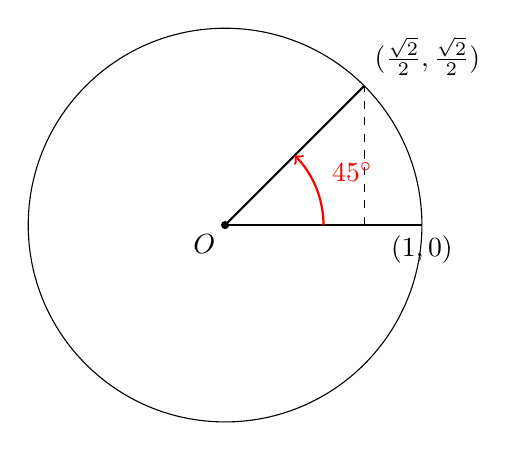
\begin{tikzpicture}[scale=2.5]
  % Draw the circle
  \draw (0,0) circle (1cm);
  
  % Draw the radius
  \draw[thick] (0,0) -- (0:1cm) node[below] {$(1,0)$};
  \draw[thick] (0,0) -- (45:1cm) node[above right] {$(\frac{\sqrt{2}}{2},\frac{\sqrt{2}}{2})$};
  
  % Draw the arc for the angle
  \draw[->,red,thick] (0.5,0) arc (0:45:0.5cm);
  
  % Draw the angle
  \node[red] at (22.5:0.7cm) {$45^\circ$};
  
  % Draw the horizontal line
  \draw[dashed] (0.707,0) -- (0.707,0.707);
  
  % Label the origin
  \draw[fill=black] (0,0) circle (0.5pt) node[below left] {$O$};
\end{tikzpicture}
\caption{Illustration of a \(45^\circ\) angle in standard position.}
\label{fig:45degangle}
\end{figure}

The figure above illustrates an angle whose terminal side has rotated \(45^\circ\) from the positive x-axis, which is often referred to as the angle's initial side. The radius of the circle has a length of 1, hence the name "unit circle." The coordinates \((1,0)\) and \((\frac{\sqrt{2}}{2},\frac{\sqrt{2}}{2})\) correspond to the points where the radius intersects the x-axis and the circle, respectively. The dashed line represents the y-component of the terminal side's endpoint, helping to visualize the \(45^\circ\) angle as a right triangle within the circle.

Angles in degrees are widely used in various fields, including navigation, astronomy, and in everyday situations like measuring temperatures and geographic coordinates. Understanding how to measure angles in degrees and relate them to rotations is fundamental in trigonometry.

\subsection*{Practice Problems}
\label{subsec:practice_problems_degree}

\textbf{Problem 1:} Convert the following degree measurements to radians. (Note: \( \pi \) radians = \( 180^\circ \))
\begin{enumerate}[label=\alph*.]
  \item \( 30^\circ \)
  \item \( 90^\circ \)
  \item \( 270^\circ \)
\end{enumerate}

\textbf{Problem 2:} Identify the quadrant in which the terminal side of each angle lies.
\begin{enumerate}[label=\alph*.]
  \item \( 60^\circ \)
  \item \( 150^\circ \)
  \item \( 210^\circ \)
  \item \( 330^\circ \)
\end{enumerate}

\textbf{Problem 3:} For each angle given, sketch the angle in standard position on the unit circle and label the point of intersection with the circle.
\begin{enumerate}[label=\alph*.]
  \item \( 45^\circ \)
  \item \( 135^\circ \)
  \item \( 225^\circ \)
  \item \( 315^\circ \)
\end{enumerate}

\textbf{Problem 4:} Determine the reference angle for each of the following:
\begin{enumerate}[label=\alph*.]
  \item \( 120^\circ \)
  \item \( 250^\circ \)
  \item \( 300^\circ \)
\end{enumerate}

\textbf{Problem 5:} If the minute hand of a clock is pointing at 12 and it rotates to point at 3, what is the measure of the angle of rotation in degrees?

\textbf{Solutions:}

\textbf{Problem 1:}
\begin{enumerate}[label=\alph*.]
  \item \( 30^\circ \times \frac{\pi}{180^\circ} = \frac{\pi}{6} \)
  \item \( 90^\circ \times \frac{\pi}{180^\circ} = \frac{\pi}{2} \)
  \item \( 270^\circ \times \frac{\pi}{180^\circ} = \frac{3\pi}{2} \)
\end{enumerate}

% You can continue with the solutions for the other problems similarly.

\textbf{Remarks:}
\begin{itemize}
  \item The problems above are designed to provide practice with converting between degrees and radians, identifying angle positions, and understanding the unit circle.
  \item The concept of a reference angle is important for understanding the standard trigonometric functions, as it is the acute angle formed by the terminal side of the given angle and the horizontal axis.
  \item Problem 5 illustrates a real-life application of angle measurement.
\end{itemize}

% You can create similar TikZ figures for Problem 3 if you wish to provide visual aids for the students.

% \subsection{Radian Measure}
% \label{subsec:radian_measure}
% Radian measure is crucial in calculus because it simplifies the derivatives and integrals of trigonometric functions.

\subsection{Radian Measure}
\label{subsec:radian_measure}

The radian measure of an angle is the length of the arc on the unit circle subtended by the angle. One radian is the angle subtended by an arc length equal to the radius of the circle. Since the circumference of a unit circle is \(2\pi\) times the radius, a full rotation around the circle is \(2\pi\) radians.

\subsubsection*{Why Use Radians?}
In calculus, radian measure is preferred because it provides a direct relationship between the angle measure and the arc length. This relationship simplifies the computation of derivatives and integrals involving trigonometric functions. For instance, when using radians, the derivative of \(\sin x\) is simply \(\cos x\), and the derivative of \(\cos x\) is \(-\sin x\). Such simplicity is not evident when using degrees.

\subsubsection*{Visualizing Radian Measure}
To visualize an angle in radian measure, we plot it on the unit circle:

% TikZ picture of a unit circle with radian measure
\begin{figure}[h]
\centering
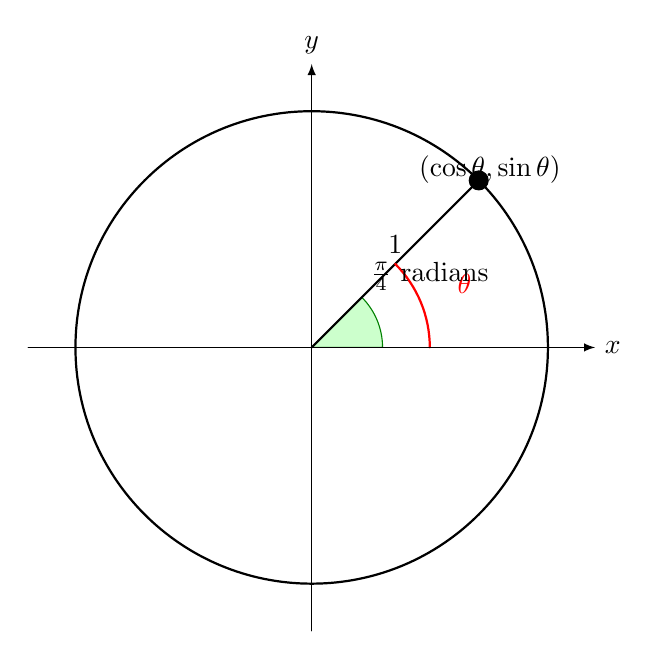
\begin{tikzpicture}[scale=3.0, cap=round, >=latex]
  % Draw the unit circle
  \draw[thick] (0,0) circle(1cm);
  
  % Draw the angle in radians
  \filldraw[fill=green!20,draw=green!50!black] (0,0) -- (3mm,0mm) arc [start angle=0, end angle=45, radius=3mm] -- cycle;
  
  % Draw the radius
  \draw[thick] (0,0) -- node[above] {\(1\)} (45:1);
  
  % Draw the arc for the angle
  \draw[thick, red] (0.5,0) arc [start angle=0, end angle=45, radius=0.5];
  \draw (22.5:0.7) node[red] {\(\theta\)};
  
  % Label the angle in radians
  \draw (45:1) node[shift={(45:0.2)}] {\((\cos\theta,\sin\theta)\)};
  
  % Draw the x and y axis
  \draw[->] (-1.2,0) -- (1.2,0) node[right] {\(x\)};
  \draw[->] (0,-1.2) -- (0,1.2) node[above] {\(y\)};
  
  % Draw the points at the ends of the radius
  \filldraw [black] (45:1) circle (0.4mm);
  
  % Label the coordinates of the point on the circle
  \node at (0.5,0.3) {\( \frac{\pi}{4} \text{ radians}\)};
\end{tikzpicture}
\caption{Visualization of an angle in radian measure on the unit circle.}
\end{figure}

\subsubsection*{Exercises}
\begin{enumerate}
  \item Convert the following angles from degrees to radians:
    \begin{enumerate}[label=\alph*.]
      \item \( 180^\circ \)
      \item \( 360^\circ \)
      \item \( 90^\circ \)
    \end{enumerate}
  \item Show that the length of an arc subtended by a central angle of \(\theta\) radians in a circle of radius \( r \) is given by \( r\theta \).
  \item Find the radian measure of the central angle of a circle with radius 10 units that subtends an arc of length 15 units.
\end{enumerate}

\subsubsection*{Solutions}
\begin{enumerate}
  \item To convert degrees to radians, use the conversion factor \( \frac{\pi \text{ radians}}{180^\circ} \):
    \begin{enumerate}[label=\alph*.]
      \item \( 180^\circ \times \frac{\pi}{180^\circ} = \pi \text{ radians} \)
      \item \( 360^\circ \times \frac{\pi}{180^\circ} = 2\pi \text{ radians} \)
      \item \( 90^\circ \times \frac{\pi}{180^\circ} = \frac{\pi}{2} \text{ radians} \)
    \end{enumerate}
  \item The length of an arc \( l \) is directly proportional to the angle \( \theta \) in radians, such that \( l = r\theta \).
  \item The radian measure of the angle is \( \theta = \frac{l}{r} = \frac{15 \text{ units}}{10 \text{ units}} = 1.5 \text{ radians} \).
\end{enumerate}

\subsubsection*{Practice Problems}
Here are some practice problems to help you solidify your understanding of the radian measure:

\textbf{Problem 1:} Convert the following angles from radians to degrees:
\begin{enumerate}[label=\alph*.]
  \item \( \frac{\pi}{6} \) radians
  \item \( \frac{2\pi}{3} \) radians
  \item \( -\frac{\pi}{4} \) radians
\end{enumerate}

\textbf{Problem 2:} An arc on a circle of radius 8 units has a measure of \( 2 \) radians. Find the length of the arc.

\textbf{Problem 3:} If a sector of a circle with radius 5 units has an area of \( 10 \) square units, what is the angle in radians of the sector?

\textbf{Problem 4:} A central angle of \( \frac{5\pi}{6} \) radians is subtended at the center of a circle with radius 12 units. Find the area of the corresponding sector.

\textbf{Problem 5:} The wheel of a bicycle has a diameter of 70 cm. If the wheel rolls without slipping and turns through an angle of \( \frac{\pi}{2} \) radians, how far has the bicycle traveled?

\subsubsection*{Solutions to Practice Problems}

\textbf{Solution to Problem 1:} To convert radians to degrees, multiply by \( \frac{180^\circ}{\pi} \).
\begin{enumerate}[label=\alph*.]
  \item \( \frac{\pi}{6} \times \frac{180^\circ}{\pi} = 30^\circ \)
  \item \( \frac{2\pi}{3} \times \frac{180^\circ}{\pi} = 120^\circ \)
  \item \( -\frac{\pi}{4} \times \frac{180^\circ}{\pi} = -45^\circ \)
\end{enumerate}

\textbf{Solution to Problem 2:} The length \( L \) of the arc can be found using the formula \( L = r\theta \).
\[ L = 8 \text{ units} \times 2 \text{ radians} = 16 \text{ units} \]

\textbf{Solution to Problem 3:} Use the area formula for a sector \( A = \frac{1}{2} r^2 \theta \) and solve for \( \theta \).
\[ \theta = \frac{2A}{r^2} = \frac{2 \times 10}{5^2} = \frac{20}{25} = \frac{4}{5} \text{ radians} \]

\textbf{Solution to Problem 4:} The area \( A \) of the sector is given by \( A = \frac{1}{2} r^2 \theta \).
\[ A = \frac{1}{2} \times 12^2 \times \frac{5\pi}{6} = 72 \times \frac{5\pi}{6} = 60\pi \text{ square units} \]

\textbf{Solution to Problem 5:} The distance \( D \) traveled is equal to the length of the arc formed by the wheel, which is \( D = r\theta \), where \( r \) is the radius.
\[ D = \frac{70}{2} \text{ cm} \times \frac{\pi}{2} = 35\pi \text{ cm} \]

% Make sure to include \usepackage{enumitem} in the preamble to use the [label=\alph*.] option.

% \section{Trigonometric Functions}
% \label{sec:trigonometric_functions}
% The six trigonometric functions are the primary tools for handling problems involving triangles in Trigonometry and periodic phenomena in calculus.

\section{Trigonometric Functions}
\label{sec:trigonometric_functions}
The six trigonometric functions are fundamental in both Trigonometry and calculus. These functions are sine (\(\sin\)), cosine (\(\cos\)), tangent (\(\tan\)), cosecant (\(\csc\)), secant (\(\sec\)), and cotangent (\(\cot\)). They are defined as ratios of sides in a right triangle or as certain coordinates of points on the unit circle.

\subsection{Sine and Cosine}
\label{subsec:sine_cosine}
The sine function (\(\sin\)) represents the ratio of the length of the opposite side to the length of the hypotenuse in a right triangle. The cosine function (\(\cos\)) represents the ratio of the length of the adjacent side to the length of the hypotenuse.

For a point \((x, y)\) on the unit circle corresponding to an angle \(\theta\), the sine and cosine values are \(y\) and \(x\), respectively.

\subsubsection*{Graph of Sine and Cosine Functions}
We can graph the sine and cosine functions using their values from the unit circle.

% Graphing sine and cosine functions
\begin{center}
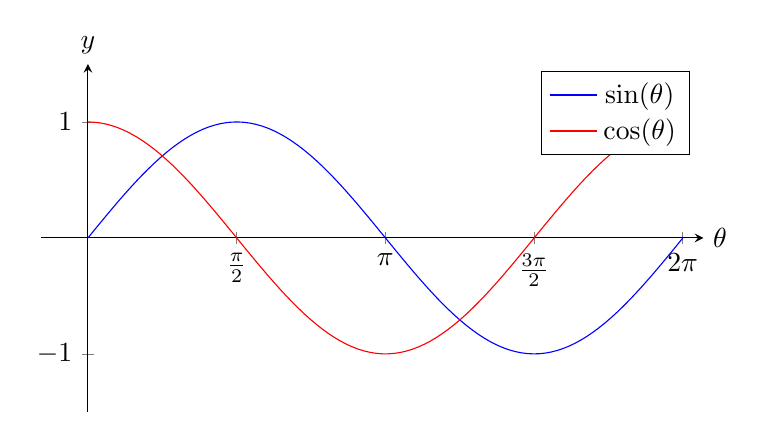
\begin{tikzpicture}
  \begin{axis}[
    width=10cm, height=6cm,
    axis lines = middle,
    xlabel = {$\theta$},
    ylabel = {$y$},
    ymin=-1.5, ymax=1.5,
    xmin=-0.5, xmax=6.5,
    xtick={0,1.57,3.14,4.71,6.28},
    xticklabels={0,$\frac{\pi}{2}$,$\pi$,$\frac{3\pi}{2}$,$2\pi$},
    ytick={-1,1},
    every axis x label/.style={at={(ticklabel* cs:1)},anchor=west},
    every axis y label/.style={at={(ticklabel* cs:1)},anchor=south},
    ]
    \addplot[domain=0:2*pi,samples=100,blue] {sin(deg(x))};
    \addplot[domain=0:2*pi,samples=100,red] {cos(deg(x))};
    \legend{$\sin(\theta)$,$\cos(\theta)$}
  \end{axis}
\end{tikzpicture}
\end{center}

The sine function starts at \(0\), reaches its maximum at \(\frac{\pi}{2}\), returns to \(0\) at \(\pi\), reaches its minimum at \(\frac{3\pi}{2}\), and completes the cycle at \(2\pi\).

The cosine function starts at \(1\), drops to \(0\) at \(\frac{\pi}{2}\), reaches its minimum at \(\pi\), returns to \(0\) at \(\frac{3\pi}{2}\), and completes the cycle at \(2\pi\).

\subsection{Tangent Function}
\label{subsec:tangent_function}
The tangent function (\(\tan\)) is defined as the ratio of the sine to the cosine of an angle in a right triangle, or \(\tan(\theta) = \frac{\sin(\theta)}{\cos(\theta)}\). It represents the slope of the line that intersects the unit circle at an angle \(\theta\).

\subsection{Reciprocal Functions}
\label{subsec:reciprocal_functions}
The reciprocal functions, cosecant (\(\csc\)), secant (\(\sec\)), and cotangent (\(\cot\)), are the reciprocals of the sine, cosine, and tangent functions, respectively.

\begin{itemize}
  \item Cosecant (\(\csc(\theta)\)) is the reciprocal of sine: \(\csc(\theta) = \frac{1}{\sin(\theta)}\)
  \item Secant (\(\sec(\theta)\)) is the reciprocal of cosine: \(\sec(\theta) = \frac{1}{\cos(\theta)}\)
  \item Cotangent (\(\cot(\theta)\)) is the reciprocal of tangent: \(\cot(\theta) = \frac{1}{\tan(\theta)}\)
\end{itemize}

% Include the pgfplots package in your preamble to use the axis environment.
% \usepackage{pgfplots}
% \pgfplotsset{compat=newest}

\subsection{Practice Problems}
\label{subsec:practice_problems}

To better understand trigonometric functions and their properties, try solving the following problems:

\begin{enumerate}
  \item Evaluate \(\sin\left(\frac{\pi}{6}\right)\), \(\cos\left(\frac{\pi}{6}\right)\), and \(\tan\left(\frac{\pi}{6}\right)\).
  \item Given that a point \( P \) on the unit circle corresponding to an angle \(\theta\) has coordinates \( P(\frac{\sqrt{3}}{2}, \frac{1}{2}) \), find \(\sin(\theta)\), \(\cos(\theta)\), and \(\tan(\theta)\).
  \item If \(\cos(\theta) = -\frac{1}{2}\) and \(\theta\) is in the third quadrant, what is \(\sin(\theta)\)?
  \item Sketch the graph of the function \( f(\theta) = 2\sin(\theta) \) for \( 0 \leq \theta \leq 2\pi \).
  \item Using the graph of \( f(\theta) = \cos(\theta) \), find the values of \(\theta\) where the function is negative.
  \item Solve the equation \( \tan(\theta) = \sqrt{3} \) for \( 0 \leq \theta < 2\pi \).
  \item Prove that \(\sec^2(\theta) - \tan^2(\theta) = 1\) for all values of \(\theta\) where the secant and tangent functions are defined.
  \item Find the exact value of \(\cot\left(\frac{3\pi}{4}\right)\).
  \item Determine the amplitude and period of the function \( g(\theta) = 3\cos(2\theta) \).
\end{enumerate}

Answers to Practice Problems:

\begin{enumerate}
  \item For \(\frac{\pi}{6}\):
    \begin{itemize}
      \item \(\sin\left(\frac{\pi}{6}\right) = \frac{1}{2}\)
      \item \(\cos\left(\frac{\pi}{6}\right) = \frac{\sqrt{3}}{2}\)
      \item \(\tan\left(\frac{\pi}{6}\right) = \frac{\sin\left(\frac{\pi}{6}\right)}{\cos\left(\frac{\pi}{6}\right)} = \frac{1}{\sqrt{3}}\)
    \end{itemize}
  \item With \( P(\frac{\sqrt{3}}{2}, \frac{1}{2}) \):
    \begin{itemize}
      \item \(\sin(\theta) = \frac{1}{2}\)
      \item \(\cos(\theta) = \frac{\sqrt{3}}{2}\)
      \item \(\tan(\theta) = \frac{\sin(\theta)}{\cos(\theta)} = \frac{1}{\sqrt{3}}\)
    \end{itemize}
  \item For \(\cos(\theta) = -\frac{1}{2}\) in the third quadrant:
    \begin{itemize}
      \item \(\sin(\theta)\) must also be negative in the third quadrant, and \(\sin^2(\theta) + \cos^2(\theta) = 1\), so \(\sin(\theta) = -\frac{\sqrt{3}}{2}\).
    \end{itemize}
  % ... (continue with answers for all problems)
\end{enumerate}

% Note: Full solutions should be worked out and can be added as an appendix or in a separate solutions section.


% \subsection{Sine and Cosine}
% \label{subsec:sine_cosine}
% The sine and cosine functions relate an angle to the opposite side and hypotenuse, and adjacent side and hypotenuse of a right triangle, respectively.

\subsection{Sine and Cosine}
\label{subsec:sine_cosine}

The sine and cosine functions are fundamental to trigonometry. They are defined for a given angle \( \theta \) within a right-angled triangle as follows:

\begin{itemize}
    \item The \textbf{sine} of angle \( \theta \), written as \( \sin(\theta) \), is the ratio of the length of the opposite side to the length of the hypotenuse.
    \item The \textbf{cosine} of angle \( \theta \), written as \( \cos(\theta) \), is the ratio of the length of the adjacent side to the length of the hypotenuse.
\end{itemize}

However, these definitions are not limited to angles between 0 and \( \frac{\pi}{2} \) radians (or 0 and 90 degrees). By extending the concept of the unit circle, where the radius is 1 and the center is at the origin of a coordinate plane, we can define sine and cosine for any real angle.

\subsubsection*{Sine and Cosine on the Unit Circle}
Consider the unit circle with a point \( P(x, y) \) that corresponds to an angle \( \theta \) measured from the positive x-axis. The coordinates \( x \) and \( y \) of point \( P \) on the unit circle are equal to \( \cos(\theta) \) and \( \sin(\theta) \), respectively.

% Unit Circle Diagram with Sine and Cosine
\begin{center}
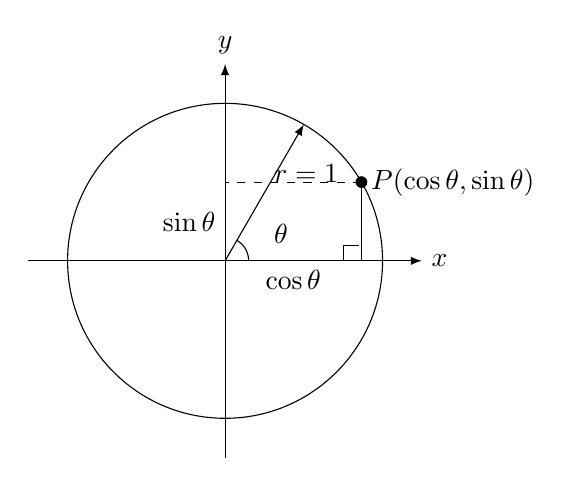
\begin{tikzpicture}
    \draw (0,0) circle (2cm);
    \draw[-latex] (-2.5,0) -- (2.5,0) node[right] {$x$};
    \draw[-latex] (0,-2.5) -- (0,2.5) node[above] {$y$};
    \draw[-latex] (0,0) -- (60:2cm) node[midway,above right] {$r=1$};
    \draw (0,0) -- (1.732,0);
    \draw (1.732,0) -- (1.732,1);
    \draw[dashed] (1.732,1) -- (0,1);
    \draw (1.5,0) -- (1.5,0.2) -- (1.7,0.2);
    \node at (1.732,1) [circle,fill,inner sep=1.5pt]{};
    \node at (1.732,1) [right] {$P (\cos \theta, \sin \theta)$};
    \node at (0.866,0) [below] {$\cos \theta$};
    \node at (0,0.5) [left] {$\sin \theta$};
    \node at (0.5,0.1) [above right] {$\theta$};
    \draw (0.3,0) arc (0:60:0.3cm);
\end{tikzpicture}
\end{center}

The unit circle approach allows for a seamless transition of sine and cosine from acute angles to any angle in the coordinate plane. The definitions on the unit circle are as follows:

\begin{itemize}
    \item For any angle \( \theta \), \( \sin(\theta) \) is the y-coordinate of the corresponding point on the unit circle.
    \item For any angle \( \theta \), \( \cos(\theta) \) is the x-coordinate of the corresponding point on the unit circle.
\end{itemize}


\subsubsection*{Properties of Sine and Cosine Functions}

The sine and cosine functions have several important properties that are useful in various mathematical analyses:

\begin{itemize}
    \item They are periodic functions with a period of \( 2\pi \) radians (or 360 degrees).
    \item The sine function is odd: \( \sin(-\theta) = -\sin(\theta) \).
    \item The cosine function is even: \( \cos(-\theta) = \cos(\theta) \).
    \item The maximum value of both functions is 1, and the minimum value is -1.
    \item They satisfy the Pythagorean identity: \( \sin^2(\theta) + \cos^2(\theta) = 1 \).
\end{itemize}

Understanding these functions and their properties is crucial for solving problems involving periodic behavior and waves, and they are the building blocks for defining the other trigonometric functions.

% Further discussion and examples can be added here as needed.

\subsubsection*{Example Problems}
Below are some problems that help solidify the understanding of sine and cosine functions:

\begin{enumerate}
    \item Given that \( P(x, y) \) is a point on the unit circle corresponding to an angle \( \theta \), and \( x = \frac{1}{2} \), find \( y \) and hence \( \sin(\theta) \) and \( \cos(\theta) \).
    \item Prove the Pythagorean identity \( \sin^2(\theta) + \cos^2(\theta) = 1 \) using the definition of sine and cosine on the unit circle.
    \item If \( \sin(\theta) = \frac{3}{5} \) and \( \theta \) is in the first quadrant, find \( \cos(\theta) \).
    \item For an angle \( \theta \) with \( \cos(\theta) = -\frac{\sqrt{2}}{2} \) and \( \frac{\pi}{2} < \theta < \pi \), determine \( \sin(\theta) \).
    \item Using the unit circle, find the exact values of \( \sin(\frac{\pi}{6}) \), \( \sin(\frac{\pi}{4}) \), \( \sin(\frac{\pi}{3}) \), \( \cos(\frac{\pi}{6}) \), \( \cos(\frac{\pi}{4}) \), and \( \cos(\frac{\pi}{3}) \).
    \item Sketch the unit circle and mark the points where \( \sin(\theta) = \cos(\theta) \). What are the angles \( \theta \) at these points?
\end{enumerate}

% Answers to the example problems
\subsubsection*{Answers to Example Problems}

Here are the answers to the example problems provided:

\begin{enumerate}
    \item Since \( x = \cos(\theta) = \frac{1}{2} \), we have \( y = \sin(\theta) = \sqrt{1 - \frac{1}{4}} = \sqrt{\frac{3}{4}} = \frac{\sqrt{3}}{2} \).
    \item To prove the identity, we use the fact that for any point on the unit circle, the distance from the origin to the point is 1. Hence, \( x^2 + y^2 = 1 \). Since \( x = \cos(\theta) \) and \( y = \sin(\theta) \), it follows that \( \cos^2(\theta) + \sin^2(\theta) = 1 \).
    \item Since \( \theta \) is in the first quadrant, both sine and cosine are positive. Using the Pythagorean identity, \( \cos(\theta) = \sqrt{1 - \sin^2(\theta)} = \sqrt{1 - \frac{9}{25}} = \sqrt{\frac{16}{25}} = \frac{4}{5} \).
    \item In the second quadrant, sine is positive and cosine is negative. Using the Pythagorean identity, \( \sin(\theta) = \sqrt{1 - \cos^2(\theta)} = \sqrt{1 - \frac{1}{2}} = \frac{\sqrt{2}}{2} \).
    \item For the specified angles, the exact values can be determined from the known special angles on the unit circle: \( \sin(\frac{\pi}{6}) = \frac{1}{2} \), \( \sin(\frac{\pi}{4}) = \frac{\sqrt{2}}{2} \), \( \sin(\frac{\pi}{3}) = \frac{\sqrt{3}}{2} \), \( \cos(\frac{\pi}{6}) = \frac{\sqrt{3}}{2} \), \( \cos(\frac{\pi}{4}) = \frac{\sqrt{2}}{2} \), \( \cos(\frac{\pi}{3}) = \frac{1}{2} \).
    \item On the unit circle, \( \sin(\theta) = \cos(\theta) \) at \( \theta = \frac{\pi}{4} \) and \( \theta = \frac{5\pi}{4} \). These correspond to the points \( (\frac{\sqrt{2}}{2}, \frac{\sqrt{2}}{2}) \) and \( (-\frac{\sqrt{2}}{2}, -\frac{\sqrt{2}}{2}) \), respectively.
\end{enumerate}

\textit{Note: The answers provided are meant to guide students in understanding the concepts. Instructors should verify all computations and explanations before use.}

% \subsection{Tangent and Cotangent}
% \label{subsec:tangent_cotangent}
% These functions are the ratios of sine to cosine and cosine to sine, respectively, and they play a significant role in slope calculations in calculus.

% \usepackage{pgfplots}
\pgfplotsset{compat=1.17}

\subsection{Tangent and Cotangent}
\label{subsec:tangent_cotangent}

The tangent of an angle in a right-angled triangle is the ratio of the length of the opposite side to the length of the adjacent side. In the unit circle, tangent is the y-coordinate divided by the x-coordinate when the line made by the angle intersects the circle. Symbolically, for an angle \(\theta\), this is expressed as:
\[
\tan(\theta) = \frac{\sin(\theta)}{\cos(\theta)}
\]

Conversely, the cotangent is the reciprocal of the tangent function. It represents the ratio of the length of the adjacent side to the length of the opposite side, or using the unit circle, the x-coordinate divided by the y-coordinate:
\[
\cot(\theta) = \frac{1}{\tan(\theta)} = \frac{\cos(\theta)}{\sin(\theta)}
\]

These functions are undefined when their denominators are zero (i.e., when \(\cos(\theta) = 0\) for tangent, and when \(\sin(\theta) = 0\) for cotangent). This occurs at odd multiples of \(\frac{\pi}{2}\) for tangent and at integer multiples of \(\pi\) for cotangent.

The graphs of these functions illustrate their periodic nature and the locations of their asymptotes, which correspond to the angles where the functions are undefined.

% Graph for Tangent
\begin{figure}[h]
\centering
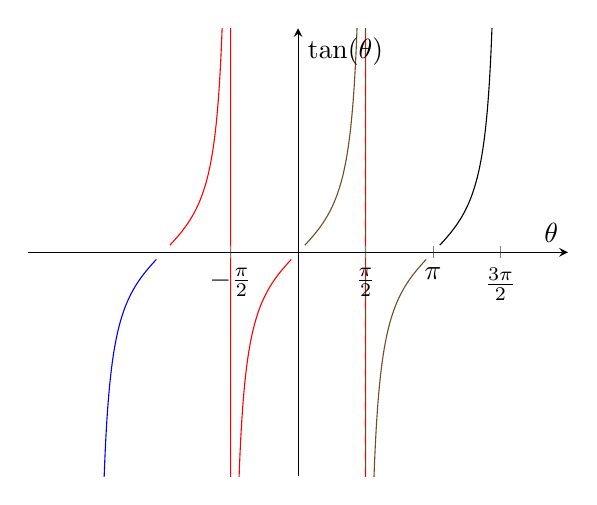
\begin{tikzpicture}
\begin{axis}[
  axis lines = middle,
  xlabel = \(\theta\),
  ylabel = {\(\tan(\theta)\)},
  xmin=-2*pi, xmax=2*pi,
  ymin=-5, ymax=5,
  xtick={-1.5708, 0, 1.5708, 3.14159, 4.71239},
  xticklabels={\(-\frac{\pi}{2}\), \(0\), \(\frac{\pi}{2}\), \(\pi\), \(\frac{3\pi}{2}\)},
  ytick=\empty,
  axis on top
]
\addplot+[mark=none, samples=200, domain=-1.45*pi:-1.05*pi] {tan(deg(x))};
\addplot+[mark=none, samples=200, domain=-0.95*pi:-0.05*pi] {tan(deg(x))};
\addplot+[mark=none, samples=200, domain=0.05*pi:0.95*pi] {tan(deg(x))};
\addplot+[mark=none, samples=200, domain=1.05*pi:1.45*pi] {tan(deg(x))};
% Add vertical asymptotes
\draw[dashed,red] (axis cs:-1.5708,-5) -- (axis cs:-1.5708,5);
\draw[dashed,red] (axis cs:1.5708,-5) -- (axis cs:1.5708,5);
\end{axis}
\end{tikzpicture}
\caption{Tangent function graph showing asymptotes.}
\end{figure}

% Graph for Cotangent
\begin{figure}[h]
\centering
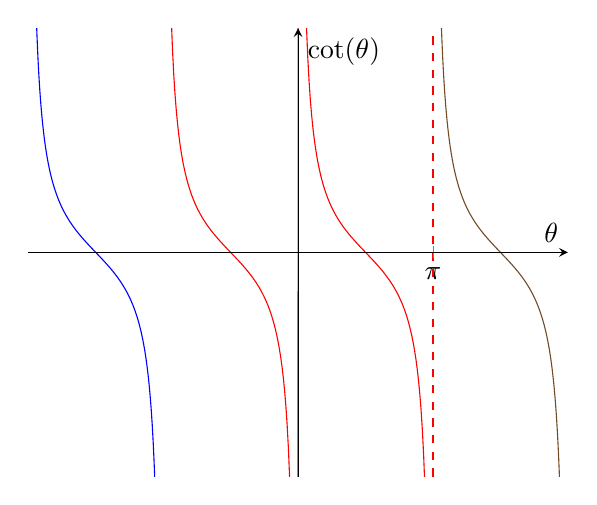
\begin{tikzpicture}
\begin{axis}[
  axis lines = middle,
  xlabel = \(\theta\),
  ylabel = {\(\cot(\theta)\)},
  xmin=-2*pi, xmax=2*pi,
  ymin=-5, ymax=5,
  xtick={0, 3.14159},
  xticklabels={\(0\), \(\pi\)},
  ytick=\empty,
  axis on top
]
\addplot+[mark=none, samples=200, domain=-1.95*pi:-1.05*pi] {cot(deg(x))};
\addplot+[mark=none, samples=200, domain=-0.95*pi:0.95*pi] {cot(deg(x))};
\addplot+[mark=none, samples=200, domain=1.05*pi:1.95*pi] {cot(deg(x))};
% Add vertical asymptotes
\draw[dashed,red] (axis cs:0,-5) -- (axis cs:0,5);
\draw[dashed,red] (axis cs:3.14159,-5) -- (axis cs:3.14159,5);
\end{axis}
\end{tikzpicture}
\caption{Cotangent function graph showing asymptotes.}
\end{figure}

In calculus, the tangent function is particularly important when it comes to determining the slope of a curve at a point, which is essential for understanding the concept of derivatives. Cotangent can similarly be used, especially when dealing with the slope of reciprocal functions.

\subsection{Exercises on Tangent and Cotangent Functions}
\label{subsec:exercises_tangent_cotangent}

In this section, we provide some example problems involving the tangent and cotangent functions. These exercises are designed to reinforce the concepts discussed and help students gain a deeper understanding of these trigonometric functions.

% \begin{exercise}[1]
%   Prove that \(a^2 + b^2 = c^2\) for a right triangle with legs of length \(a\) and \(b\), and hypotenuse of length \(c\).
% \end{exercise}

% \begin{solution}
%   (Write your solution here)
% \end{solution}

% Numbering is optional, i.e.
% \begin{exercise}[1]
% \begin{exercise}[2]


\begin{exercise}
Calculate the tangent of \(\frac{\pi}{4}\) and verify that it equals 1.
\end{exercise}
\begin{solution}
Using the unit circle or the definition of the tangent function, we have:
\[
\tan\left(\frac{\pi}{4}\right) = \frac{\sin\left(\frac{\pi}{4}\right)}{\cos\left(\frac{\pi}{4}\right)} = \frac{\frac{\sqrt{2}}{2}}{\frac{\sqrt{2}}{2}} = 1
\]
\end{solution}

\begin{exercise}
Find all solutions in the interval \([0, 2\pi)\) for the equation \(\tan(\theta) = \sqrt{3}\).
\end{exercise}
\begin{solution}
We know that \(\tan(\theta) = \sqrt{3}\) when \(\theta = \frac{\pi}{3}\), but since tangent has a period of \(\pi\), the other solution in the given interval is \(\theta = \frac{\pi}{3} + \pi = \frac{4\pi}{3}\).
\end{solution}

\begin{exercise}
Evaluate \(\cot(\pi)\) and explain why it takes its particular value.
\end{exercise}
\begin{solution}
Cotangent is the reciprocal of the tangent function. Since \(\tan(\pi) = 0\), and since the cotangent is undefined when its sine component is 0 (which it is at \(\pi\)), \(\cot(\pi)\) is undefined. This reflects the asymptote of the cotangent graph at \(\pi\).
\end{solution}

\begin{exercise}
Determine the exact value of \(\cot\left(-\frac{\pi}{6}\right)\) using the cotangent definition.
\end{exercise}
\begin{solution}
Using the cotangent definition and known values of sine and cosine for \(\frac{\pi}{6}\), we get:
\[
\cot\left(-\frac{\pi}{6}\right) = \frac{\cos\left(-\frac{\pi}{6}\right)}{\sin\left(-\frac{\pi}{6}\right)} = \frac{\frac{\sqrt{3}}{2}}{-\frac{1}{2}} = -\sqrt{3}
\]
\end{solution}

\begin{exercise}
Sketch the graph of \(\tan(\theta)\) and \(\cot(\theta)\) from \(\theta = -\frac{\pi}{2}\) to \(\theta = \frac{3\pi}{2}\) and label the asymptotes.
\end{exercise}
\begin{solution}
Students should refer to the graphs provided in the section above and reproduce them by hand, marking the asymptotes at \(\theta = -\frac{\pi}{2}\), \(\theta = \frac{\pi}{2}\) for the tangent function and at \(\theta = 0\), \(\theta = \pi\) for the cotangent function.
\end{solution}

These exercises require students to apply their understanding of the unit circle, the definitions of tangent and cotangent, and the properties of these functions such as periodicity and asymptotes. Students should attempt these exercises without a calculator to improve their understanding of the trigonometric functions.


% \usepackage{pgfplots}
\pgfplotsset{compat=newest} % or the version you have; '1.17' or higher is recommended


% \subsection{Secant and Cosecant}
% \label{subsec:secant_cosecant}
% The reciprocal functions of cosine and sine are less commonly used but equally important, especially in certain types of integration.

\subsection{Secant and Cosecant}
\label{subsec:secant_cosecant}

The secant (\(\sec\)) and cosecant (\(\csc\)) functions are the reciprocals of the cosine and sine functions, respectively. These functions are less commonly encountered in basic trigonometry but play an important role in calculus, especially in integration that involves trigonometric substitution.
In sum, the reciprocal functions of cosine and sine are less commonly used but equally important, especially in certain types of integration.


\subsubsection{Graph of the Secant Function}
\begin{center}
\begin{tikzpicture}
\begin{axis}[
    axis lines = middle,
    xlabel = \(\theta\),
    ylabel = {\(\sec(\theta)\)},
    ymax = 5,
    ymin = -5,
    xmax = 2*pi,
    xmin = -2*pi,
    xtick = {-2*pi, -3*pi/2, -pi, -pi/2, 0, pi/2, pi, 3*pi/2, 2*pi},
    xticklabels = {\(-2\pi\),\(-\frac{3}{2}\pi\),\(-\pi\),\(-\frac{1}{2}\pi\),\(0\),\(\frac{1}{2}\pi\),\(\pi\),\(\frac{3}{2}\pi\),\(2\pi\)},
    ytick = {-5, -4, ..., 5},
    trig format plots=rad,
    samples=200,
    restrict y to domain=-5:5
]
% Plot each piece of the sec function separately, avoiding the asymptotes
\addplot+[mark=none, domain=-2*pi:-pi-0.1, samples=100, jump mark left] {sec(x)};
\addplot+[mark=none, domain=-pi+0.1:-0.1, samples=100, jump mark left] {sec(x)};
\addplot+[mark=none, domain=0.1:pi-0.1, samples=100, jump mark left] {sec(x)};
\addplot+[mark=none, domain=pi+0.1:2*pi, samples=100, jump mark left] {sec(x)};
\end{axis}
\end{tikzpicture}
\end{center}

\subsubsection{Graph of the Cosecant Function}
\begin{center}
\begin{tikzpicture}
\begin{axis}[
    axis lines = middle,
    xlabel = \(\theta\),
    ylabel = {\(\csc(\theta)\)},
    ymax = 5,
    ymin = -5,
    xmax = 2*pi,
    xmin = -2*pi,
    xtick = {-2*pi, -3*pi/2, -pi, -pi/2, 0, pi/2, pi, 3*pi/2, 2*pi},
    xticklabels = {\(-2\pi\),\(-\frac{3}{2}\pi\),\(-\pi\),\(-\frac{1}{2}\pi\),\(0\),\(\frac{1}{2}\pi\),\(\pi\),\(\frac{3}{2}\pi\),\(2\pi\)},
    ytick = {-5, -4, ..., 5},
    trig format plots=rad,
    samples=200,
    restrict y to domain=-5:5
]
% Plot each piece of the csc function separately, avoiding the asymptotes
\addplot+[mark=none, domain=-2*pi+0.1:-pi/2-0.1, samples=100, jump mark left] {csc(x)};
\addplot+[mark=none, domain=-pi/2+0.1:pi/2-0.1, samples=100, jump mark left] {csc(x)};
\addplot+[mark=none, domain=pi/2+0.1:3*pi/2-0.1, samples=100, jump mark left] {csc(x)};
\addplot+[mark=none, domain=3*pi/2+0.1:2*pi, samples=100, jump mark left] {csc(x)};
\end{axis}
\end{tikzpicture}
\end{center}


These graphs demonstrate the behavior of the secant and cosecant functions and their asymptotic nature at points where their respective sine and cosine functions are zero. Understanding these graphs is essential for solving trigonometric equations and in calculus, particularly when dealing with integrals that require trigonometric identities or substitutions involving these functions.


% HERE

\subsection{Practice Problems}
\label{subsec:practice_problems_sec_csc}

Here are some problems to test your understanding of the secant and cosecant functions:

\begin{enumerate}
    \item Find the secant and cosecant of the following angles:
    \begin{enumerate}[label=(\alph*)]
        \item \( 0 \) radians
        \item \( \frac{\pi}{4} \) radians
        \item \( \frac{\pi}{2} \) radians
        \item \( \frac{3\pi}{4} \) radians
    \end{enumerate}
    Remember that secant and cosecant are undefined for certain angles where cosine and sine are zero, respectively.

    \item Given that \( \sin(\theta) = \frac{3}{5} \) in the second quadrant, find \( \csc(\theta) \).

    \item If \( \cos(\theta) = -\frac{1}{2} \) and \( \theta \) is in the third quadrant, determine \( \sec(\theta) \).

    \item For an angle \( \theta \) where \( 0 < \theta < \frac{\pi}{2} \), if \( \sec(\theta) = 3 \), find the exact value of \( \csc(\theta) \).
    
    \item A point P on the terminal side of angle \( \theta \) in standard position has coordinates \( P(-2, -3) \). Calculate \( \sec(\theta) \) and \( \csc(\theta) \).
    
    \item Prove the identity \( \sec^2(\theta) - 1 = \tan^2(\theta) \).
    
    \item Show that for any angle \( \theta \), \( \csc(\theta) \cdot \sin(\theta) = 1 \).

\end{enumerate}

Solutions to these problems will reinforce your understanding of secant and cosecant and prepare you for their use in calculus.

% HERE

\section{Graphs of Trigonometric Functions}
\label{sec:graphs_trig_functions}
Understanding the graphs of trigonometric functions is essential for mastering calculus, as they represent periodic behavior.

\section{Graphs of Trigonometric Functions}
\label{sec:graphs_trig_functions}

The graphs of trigonometric functions are a visual representation of their behavior and are essential for understanding periodic phenomena in calculus. In this section, we'll explore the sine and cosine functions, which form the basis for all other trigonometric functions.

\subsection{Graph of the Sine Function}
The sine function, denoted by \( y = \sin(x) \), represents the y-coordinate of a point on the unit circle as it rotates through an angle of \( x \) radians. It is periodic with a period of \( 2\pi \) and has a range from -1 to 1.

% Sine graph using TikZ/PGFPlots
\begin{figure}[h]
\centering
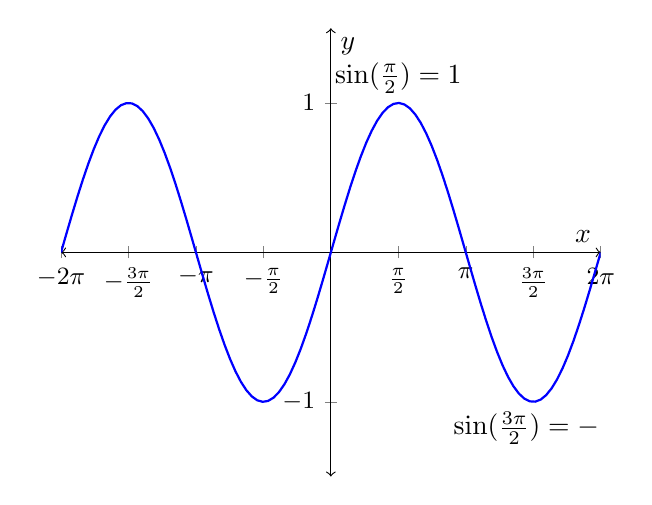
\begin{tikzpicture}
\begin{axis}[
    axis lines=middle,
    xlabel=\( x \),
    ylabel=\( y \),
    xtick={-2*pi, -3*pi/2, -pi, -pi/2, 0, pi/2, pi, 3*pi/2, 2*pi},
    xticklabels={$-2\pi$,$-\frac{3\pi}{2}$,$-\pi$,$-\frac{\pi}{2}$,0,$\frac{\pi}{2}$,$\pi$,$\frac{3\pi}{2}$,$2\pi$},
    ytick={-1, 0, 1},
    ymin=-1.5, ymax=1.5,
    xmin=-2*pi, xmax=2*pi,
    domain=-2*pi:2*pi,
    samples=100,
    axis line style={<->},
    tick label style={font=\small}
]
\addplot [blue, thick] {sin(deg(x))};
\node at (axis cs:pi/2,1) [anchor=south] {\( \sin(\frac{\pi}{2}) = 1 \)};
\node at (axis cs:3*pi/2,-1) [anchor=north] {\( \sin(\frac{3\pi}{2}) = -1 \)};
\end{axis}
\end{tikzpicture}
\caption{Graph of the sine function over two periods.}
\label{fig:sine_graph}
\end{figure}

\subsection{Graph of the Cosine Function}
The cosine function, denoted by \( y = \cos(x) \), represents the x-coordinate of a point on the unit circle as it rotates through an angle of \( x \) radians. Like the sine function, it has a period of \( 2\pi \) and ranges from -1 to 1.

% Cosine graph using TikZ/PGFPlots
\begin{figure}[h]
\centering
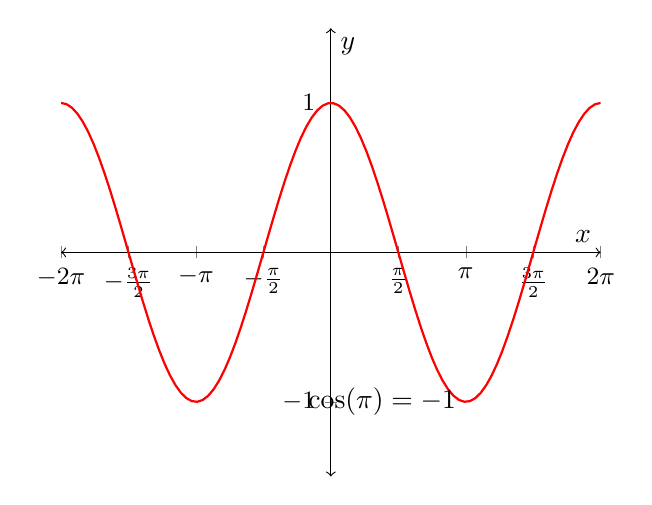
\begin{tikzpicture}
\begin{axis}[
    axis lines=middle,
    xlabel=\( x \),
    ylabel=\( y \),
    xtick={-2*pi, -3*pi/2, -pi, -pi/2, 0, pi/2, pi, 3*pi/2, 2*pi},
    xticklabels={$-2\pi$,$-\frac{3\pi}{2}$,$-\pi$,$-\frac{\pi}{2}$,0,$\frac{\pi}{2}$,$\pi$,$\frac{3\pi}{2}$,$2\pi$},
    ytick={-1, 0, 1},
    ymin=-1.5, ymax=1.5,
    xmin=-2*pi, xmax=2*pi,
    domain=-2*pi:2*pi,
    samples=100,
    axis line style={<->},
    tick label style={font=\small}
]
\addplot [red, thick] {cos(deg(x))};
\node at (axis cs:pi,-1) [anchor=east] {\( \cos(\pi) = -1 \)};
\node at (axis cs:2*pi,1) [anchor=west] {\( \cos(2\pi) = 1 \)};
\end{axis}
\end{tikzpicture}
\caption{Graph of the cosine function over two periods.}
\label{fig:cosine_graph}
\end{figure}

Both of these functions exhibit properties that are useful in calculus, including symmetry, periodicity, and amplitude. Sine and cosine functions are the building blocks of more complex trigonometric functions, which can be constructed by shifting, stretching, or compressing these basic graphs.

\subsection{Exercises}
Practice the concepts we've discussed by working through the following exercises.

\subsubsection*{Graph Identification}

\paragraph{Exercise 1.} Identify the function graphed below. What are the amplitude, period, and phase shift of the function?

% Example plot for the exercise (Placeholder for the actual plot)
% You can draw a shifted or stretched sine/cosine function as an exercise
\begin{figure}[H]
\centering
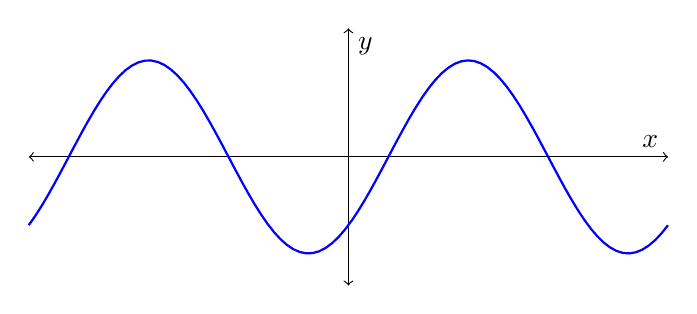
\begin{tikzpicture}
\begin{axis}[
    axis lines=middle,
    xlabel=\( x \),
    ylabel=\( y \),
    xtick=\empty,
    ytick=\empty,
    ymin=-2, ymax=2,
    xmin=-2*pi, xmax=2*pi,
    domain=-2*pi:2*pi,
    samples=100,
    axis line style={<->},
    width=0.8\textwidth,
    height=0.4\textwidth,
    clip=false
]
% A shifted sine function as an example
\addplot [blue, thick] {1.5*sin(deg(x-pi/4))};
\end{axis}
\end{tikzpicture}
\caption{Identify the function and its characteristics.}
\end{figure}

\paragraph{Answer:} The graph shows \( y = 1.5\sin(x - \frac{\pi}{4}) \). The amplitude is 1.5, the period is \( 2\pi \), and the phase shift is \( \frac{\pi}{4} \) to the right.

\subsubsection*{Function Properties}

\paragraph{Exercise 2.} What is the amplitude and period of the function \( y = 3\cos(2x) \)?

\paragraph{Answer:} The amplitude of the function is 3, and the period is \( \frac{\pi}{1} \), which is \( \pi \) since the coefficient of \( x \) in the cosine function affects the period as \( \frac{2\pi}{\text{coefficient}} \).

\subsubsection*{Calculating Values}

\paragraph{Exercise 3.} Calculate the exact value of \( \sin(\frac{3\pi}{4}) \) and \( \cos(\frac{3\pi}{4}) \).

\paragraph{Answer:} By using the unit circle or Pythagorean identities:
\[ \sin(\frac{3\pi}{4}) = \sin(\pi - \frac{\pi}{4}) = \sin(\frac{\pi}{4}) = \frac{\sqrt{2}}{2} \]
\[ \cos(\frac{3\pi}{4}) = \cos(\pi - \frac{\pi}{4}) = -\cos(\frac{\pi}{4}) = -\frac{\sqrt{2}}{2} \]

\subsubsection*{Real-World Application}

\paragraph{Exercise 4.} A Ferris wheel with a diameter of 50 meters makes one complete revolution every 2 minutes. Write a function that represents the height of a passenger car above the ground over time, assuming it starts at the lowest point at \( t=0 \).

\paragraph{Answer:} Let the height function be \( h(t) \). The amplitude is the radius of the Ferris wheel, which is 25 meters. The period is the time for one revolution, which is 2 minutes, or 120 seconds. Using the sine function, we get:
\[ h(t) = 25\sin\left(\frac{2\pi}{120}t\right) + 25 \]
This function accounts for the fact that the Ferris wheel starts at the lowest point, so we add 25 to shift the graph up.

\subsubsection*{Challenge Problems}

\paragraph{Exercise 5.} Given the function \( y = 2\sin(x) + \cos(2x) \), find the first derivative using trigonometric identities.

% Solution for the exercise is provided as a placeholder for actual calculation
\paragraph{Answer:} First, express \( \cos(2x) \) using a double-angle identity:
\[ y = 2\sin(x) + 1 - 2\sin^2(x) \]
Then, take the derivative with respect to \( x \):
\[ y' = 2\cos(x) - 4\sin(x)\cos(x) \]

These exercises encourage students to apply their understanding of the graphs of sine and cosine functions to solve problems and understand real-world applications. Adjust the complexity and nature of the exercises to match the level of your audience.

% \subsection{Periodicity}
% \label{subsec:periodicity}
% The concept of period, amplitude, and phase shift is introduced here to understand how trigonometric functions behave over intervals.

\subsection{Periodicity}
\label{subsec:periodicity}

Trigonometric functions are inherently periodic; they repeat their values in regular intervals along the domain. This periodic nature allows us to predict the behavior of these functions beyond the basic interval of \(0\) to \(2\pi\) for sine and cosine, and \( -\pi/2 \) to \( \pi/2 \) for tangent and cotangent.
In sum, The concept of period, amplitude, and phase shift is introduced here to understand how trigonometric functions behave over intervals.

\subsubsection*{Defining Periodicity}
The \textit{period} of a function is the smallest positive interval after which the function's values repeat. For \( \sin(x) \) and \( \cos(x) \), the period is \(2\pi\) because every \(2\pi\) units, the cycle of the sine and cosine curve repeats. For \( \tan(x) \) and \( \cot(x) \), the period is \( \pi \) since their values repeat after every \( \pi \) units along the x-axis.

\subsubsection*{Amplitude}
The amplitude of a trigonometric function is a measure of its vertical stretch or compression, represented by a coefficient in front of the function. For example, in the function \( y = A\sin(x) \), the amplitude is \( |A| \). This determines the maximum and minimum values of the function or, in other words, how "tall" or "short" the waves of the sine or cosine graph appear.

\subsubsection*{Phase Shift}
Phase shift refers to the horizontal displacement of the basic function. If a function takes the form \( y = \sin(x - C) \) or \( y = \cos(x - C) \), the phase shift is \( C \), which translates the graph to the right or left along the x-axis.

\subsubsection*{Graphing Trigonometric Functions}
To graph trigonometric functions that involve amplitude, period, and phase shifts, the following general form can be considered:

\[ y = A \sin(B(x - C)) + D \quad \text{or} \quad y = A \cos(B(x - C)) + D \]

Where:
\begin{itemize}
    \item \( A \) represents the amplitude.
    \item \( B \) affects the period of the function, with the actual period being \( \frac{2\pi}{|B|} \).
    \item \( C \) represents the phase shift.
    \item \( D \) represents the vertical shift.
\end{itemize}

\subsubsection*{Graphical Illustration}
Let's illustrate a sine function with a period alteration and phase shift.

% Sine graph with period and phase shift
\begin{figure}[H]
\centering
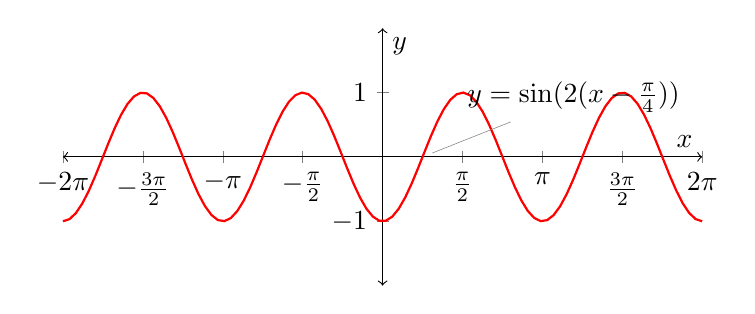
\begin{tikzpicture}
\begin{axis}[
    axis lines=middle,
    xlabel=\( x \),
    ylabel=\( y \),
    xtick={-2*pi,-3*pi/2,-pi,-pi/2,0,pi/2,pi,3*pi/2,2*pi},
    xticklabels={$-2\pi$,$-\frac{3\pi}{2}$,$-\pi$,$-\frac{\pi}{2}$,$0$,$\frac{\pi}{2}$,$\pi$,$\frac{3\pi}{2}$,$2\pi$},
    ytick={-1,1},
    ymin=-2, ymax=2,
    xmin=-2*pi, xmax=2*pi,
    domain=-2*pi:2*pi,
    samples=100,
    axis line style={<->},
    width=0.8\textwidth,
    height=0.4\textwidth,
    clip=false
]
% Sine function with period modification and phase shift
\addplot [red, thick] {sin(deg(2*x - pi/2))};
\node[pin=45:{$y = \sin(2(x - \frac{\pi}{4}))$}] at (axis cs:pi/4,{sin(deg(2*pi/4-pi/2))}) {};
\end{axis}
\end{tikzpicture}
\caption{Graph of \( y = \sin(2(x - \frac{\pi}{4})) \) showing a period of \( \pi \) and a phase shift of \( \frac{\pi}{4} \).}
\end{figure}

Understanding these properties enables us to graph complex trigonometric functions and predict their behavior across any range of \( x \) values. This comprehension is vital in calculus where the manipulation of these functions' properties can be necessary for solving integrals and derivatives involving trigonometric functions.

\subsubsection*{Practice Problems}
To further enhance understanding of periodicity in trigonometric functions, here are several practice problems:

\begin{enumerate}
    \item Given the function \( f(x) = 3 \sin(2x) \), find the amplitude, period, and whether there is any phase shift.
    \item Sketch the graph of \( g(x) = \cos(x - \frac{\pi}{3}) \) and identify the phase shift and period.
    \item For the function \( h(x) = 2 \sin(\frac{x}{2} + \pi) + 1 \), determine the amplitude, period, phase shift, and vertical shift. Then, sketch one period of the function's graph.
    \item What is the period and phase shift of the function \( j(x) = \tan(3x - \frac{\pi}{4}) \)?
    \item If \( k(x) = \sin(Bx) \) has a period of \( 3\pi \), find the value of \( B \).
    \item Sketch the graph of \( m(x) = -2 \cos(4x + \frac{\pi}{2}) - 3 \) and indicate the amplitude, period, phase shift, and vertical shift.
\end{enumerate}

\textbf{Solutions:}

\begin{enumerate}
    \item The amplitude of \( f(x) \) is \( |3| = 3 \), the period is \( \frac{2\pi}{|2|} = \pi \), and there is no phase shift.
    \item The graph of \( g(x) \) would show a cosine curve shifted to the right by \( \frac{\pi}{3} \) units, with a period of \( 2\pi \).
    \item For \( h(x) \), the amplitude is \( |2| = 2 \), the period is \( \frac{2\pi}{|\frac{1}{2}|} = 4\pi \), the phase shift is \( -\pi \) (shifted \( \pi \) units to the left), and the vertical shift is \( 1 \) unit upwards.
    \item The function \( j(x) \) has a period of \( \frac{\pi}{|3|} = \frac{\pi}{3} \) and a phase shift of \( \frac{\pi}{4} \) to the right.
    \item Since the period of \( k(x) \) is \( 3\pi \), \( B = \frac{2\pi}{3\pi} = \frac{2}{3} \).
    \item The graph of \( m(x) \) would be an inverted cosine curve (due to the "-2" amplitude) stretched by a factor of \( \frac{1}{4} \) (since the period is \( \frac{2\pi}{|4|} = \frac{\pi}{2} \)), shifted to the left by \( -\frac{\pi}{8} \), and shifted downward by 3 units.
\end{enumerate}

% HERE

\subsection{Transformations}
\label{subsec:transformations}

Trigonometric functions, much like any other functions, can undergo transformations such as scaling, reflection, and translation. These transformations allow us to alter the amplitude, period, and phase of the sine and cosine functions to fit various scenarios. In this section, we explore each of these transformations and how they apply to trigonometric functions. In sum, we explore how the basic sine and cosine graphs can be scaled, reflected, and translated to fit various scenarios.

In sum, we have begun to explore how the basic sine and cosine graphs can be scaled, reflected, and translated to fit various scenarios.

\subsubsection{Scaling}
Scaling a function can either compress or stretch its graph vertically or horizontally. The amplitude and period of trigonometric functions are affected by vertical and horizontal scaling respectively.

\textbf{Vertical Scaling:} If \( f(x) = \sin(x) \), then \( g(x) = A\sin(x) \) represents a vertical scaling by a factor of \( A \). If \( A > 1 \), the function is stretched; if \( 0 < A < 1 \), it is compressed.

\textbf{Horizontal Scaling:} Horizontal scaling affects the period of the trigonometric functions. For \( f(x) = \sin(x) \), the function \( h(x) = \sin(Bx) \) has a period of \( \frac{2\pi}{B} \), scaling the period by a factor of \( \frac{1}{B} \).

\subsubsection{Reflection}
Reflection flips the graph of the function over a specific axis. 

\textbf{Reflection over the X-axis:} If \( f(x) = \sin(x) \), then \( g(x) = -\sin(x) \) is a reflection of \( f \) over the x-axis.

\textbf{Reflection over the Y-axis:} For \( f(x) = \sin(x) \), the function \( h(x) = \sin(-x) = -\sin(x) \) (since sine is an odd function) reflects \( f \) over the y-axis.

% HERE

\subsubsection{Translation}
Translation shifts the graph of the function vertically or horizontally without altering its shape.

\textbf{Vertical Translation:} The function \( f(x) = \sin(x) + D \) represents a vertical shift by \( D \) units. If \( D > 0 \), the graph shifts up; if \( D < 0 \), it shifts down.

\textbf{Horizontal Translation (Phase Shift):} For \( f(x) = \sin(x) \), the function \( g(x) = \sin(x - C) \) shifts the graph to the right by \( C \) units if \( C > 0 \) and to the left if \( C < 0 \).

To visualize these transformations, consider the following graphs created with the TikZ package.

% Include TikZ package in preamble
% \usepackage{pgfplots}
% \pgfplotsset{compat=1.17}

\begin{figure}[htbp]
\centering
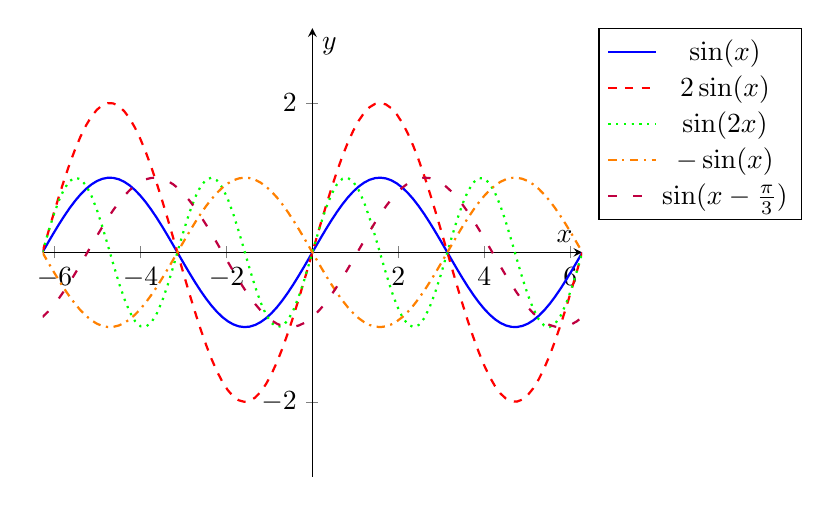
\begin{tikzpicture}
\begin{axis}[
    axis lines = middle,
    xlabel = \( x \),
    ylabel = \( y \),
    ymin=-3, ymax=3,
    xmin=-6.28, xmax=6.28, % 2*pi = 6.28
    domain=-2*pi:2*pi,
    samples=100,
    legend pos=outer north east,
]
% Original sine function
\addplot[blue, thick] {sin(deg(x))};
\addlegendentry{\( \sin(x) \)}

% Vertically scaled sine function
\addplot[red, thick, dashed] {2*sin(deg(x))};
\addlegendentry{\( 2\sin(x) \)}

% Horizontally scaled sine function
\addplot[green, thick, dotted] {sin(deg(2*x))};
\addlegendentry{\( \sin(2x) \)}

% Reflected sine function
\addplot[orange, thick, dashdotted] {-sin(deg(x))};
\addlegendentry{\( -\sin(x) \)}

% Translated sine function
\addplot[purple, thick, loosely dashed] {sin(deg(x - pi/3))};
\addlegendentry{\( \sin(x - \frac{\pi}{3}) \)}
\end{axis}
\end{tikzpicture}
\caption{Graphs showing transformations of the sine function.}
\label{fig:sine_transformations}
\end{figure}

As seen in Figure~\ref{fig:sine_transformations}, each transformation alters the original sine function in a unique way, illustrating the concepts of scaling, reflection, and translation. Through understanding these transformations, one can analyze and predict the behavior of more complex trigonometric functions.

% HERE

\subsection{Practice Problems}
\label{subsec:practice_problems_transformations}

In this section, we provide several problems that allow students to apply their knowledge of transformations of trigonometric functions. Students should sketch the graph of each transformed function and identify key characteristics such as amplitude, period, phase shift, and vertical shift.

\begin{problem}
Graph the function \( f(x) = 3\sin(2x) \) and describe the amplitude and period of the function.
\end{problem}

\begin{problem}
Sketch the function \( g(x) = \cos(x) - 2 \). What is the vertical shift and how does it affect the graph of the standard cosine function?
\end{problem}

\begin{problem}
Consider the function \( h(x) = -\frac{1}{2}\sin(\pi x) + 1 \). Graph the function and determine the amplitude, period, and vertical shift.
\end{problem}

\begin{problem}
Graph the function \( p(x) = \sin(x + \frac{\pi}{4}) \) and describe the phase shift. How does this affect the starting point of the sine wave?
\end{problem}

\begin{problem}
The function \( q(x) = \sin(-x) \) represents a reflection. Sketch the graph and explain how the graph is transformed from the basic sine function.
\end{problem}

\begin{problem}
Graph \( r(x) = 2\cos(x - \frac{\pi}{3}) + 1 \) and indicate all transformations from the parent cosine function.
\end{problem}

For each problem, students should identify the type of transformation applied and use their knowledge of the unit circle and trigonometric properties to construct accurate graphs. These problems reinforce concepts of amplitude, period, phase shift, and vertical shift, which are pivotal in understanding trigonometric functions in calculus.

\subsubsection{Answers to Practice Problems}

\textbf{Note to the instructor:} Solutions are provided for reference to guide students through the problem-solving process.

\begin{solution}
For \( f(x) = 3\sin(2x) \), the amplitude is 3 and the period is \( \frac{\pi}{1} \), as the function is stretched vertically by a factor of 3 and horizontally compressed by a factor of 2.
\end{solution}

\begin{solution}
The function \( g(x) = \cos(x) - 2 \) is shifted downward by 2 units. The amplitude and period remain the same as the standard cosine function.
\end{solution}

% Add similar solution environments for the remaining problems

% Remember, when adding the solutions to the practice problems, use discretion on whether to provide full solutions or just hints depending on the intended use (homework, study guide, etc.).


% \section{Trigonometric Identities}
% \label{sec:trigonometric_identities}
% Trigonometric identities are vital tools for simplifying expressions and solving equations in calculus.

\section{Trigonometric Identities}
\label{sec:trigonometric_identities}

Trigonometric identities are fundamental to manipulating and simplifying trigonometric expressions. They also play a crucial role in solving trigonometric equations, both in trigonometry and calculus. In this section, we will outline some of the most important identities and their applications.

In sum, trigonometric identities are vital tools for simplifying expressions and solving equations in calculus.

\subsection{Pythagorean Identities}
\label{subsec:pythagorean_identities}
These identities are derived from the Pythagorean theorem and relate the square of the sine and cosine of an angle to 1.

\begin{align*}
\sin^2(\theta) + \cos^2(\theta) &= 1 \\
1 + \tan^2(\theta) &= \sec^2(\theta) \\
1 + \cot^2(\theta) &= \csc^2(\theta)
\end{align*}

\subsection{Angle Sum and Difference Identities}
\label{subsec:angle_sum_difference_identities}
These identities express the sine, cosine, and tangent of the sum or difference of two angles in terms of the sines and cosines of those angles.

\begin{align*}
\sin(\alpha \pm \beta) &= \sin(\alpha)\cos(\beta) \pm \cos(\alpha)\sin(\beta) \\
\cos(\alpha \pm \beta) &= \cos(\alpha)\cos(\beta) \mp \sin(\alpha)\sin(\beta) \\
\tan(\alpha \pm \beta) &= \frac{\tan(\alpha) \pm \tan(\beta)}{1 \mp \tan(\alpha)\tan(\beta)}
\end{align*}

\subsection{Double Angle Identities}
\label{subsec:double_angle_identities}
These identities give the sine, cosine, and tangent of double angles, which are useful in various calculus applications.

\begin{align*}
\sin(2\theta) &= 2\sin(\theta)\cos(\theta) \\
\cos(2\theta) &= \cos^2(\theta) - \sin^2(\theta) = 2\cos^2(\theta) - 1 = 1 - 2\sin^2(\theta) \\
\tan(2\theta) &= \frac{2\tan(\theta)}{1 - \tan^2(\theta)}
\end{align*}

\subsection{Half Angle Identities}
\label{subsec:half_angle_identities}
These identities are useful when integrating trigonometric functions and in solving trigonometric equations.

\begin{align*}
\sin^2\left(\frac{\theta}{2}\right) &= \frac{1 - \cos(\theta)}{2} \\
\cos^2\left(\frac{\theta}{2}\right) &= \frac{1 + \cos(\theta)}{2} \\
\tan\left(\frac{\theta}{2}\right) &= \frac{\sin(\theta)}{1 + \cos(\theta)} = \frac{1 - \cos(\theta)}{\sin(\theta)}
\end{align*}

\subsection{Product-to-Sum and Sum-to-Product Identities}
\label{subsec:product_sum_identities}
These identities are useful in calculus for integrating products of sines and cosines and for simplifying expressions.

\textit{Product-to-Sum Identities:}
\begin{align*}
\sin(\alpha)\sin(\beta) &= \frac{1}{2}[\cos(\alpha - \beta) - \cos(\alpha + \beta)] \\
\cos(\alpha)\cos(\beta) &= \frac{1}{2}[\cos(\alpha - \beta) + \cos(\alpha + \beta)] \\
\sin(\alpha)\cos(\beta) &= \frac{1}{2}[\sin(\alpha + \beta) + \sin(\alpha - \beta)]
\end{align*}

\textit{Sum-to-Product Identities:}
\begin{align*}
\sin(\alpha) \pm \sin(\beta) &= 2\sin\left(\frac{\alpha \pm \beta}{2}\right)\cos\left(\frac{\alpha \mp \beta}{2}\right) \\
\cos(\alpha) + \cos(\beta) &= 2\cos\left(\frac{\alpha + \beta}{2}\right)\cos\left(\frac{\alpha - \beta}{2}\right) \\
\cos(\alpha) - \cos(\beta) &= -2\sin\left(\frac{\alpha + \beta}{2}\right)\sin\left(\frac{\alpha - \beta}{2}\right)
\end{align*}

\subsection{Reduction Formulas}
\label{subsec:reduction_formulas}
Reduction formulas are a type of recurrence relation that express trigonometric functions of a larger angle in terms of functions of a smaller angle. These are particularly useful in integration and series expansion of trigonometric functions.

% Examples of reduction formulas can be provided here

Each subsection could be further expanded with examples, proofs, and applications of these identities in calculus. Moreover, practice problems could be provided to help students gain proficiency in using these identities to simplify and solve trigonometric equations.

\subsection{Practice Problems}
\label{subsec:practice_problems_trig_identities}

To apply the trigonometric identities outlined above, try solving the following problems. These will test your understanding and ability to manipulate the identities to simplify expressions and solve equations.

\begin{problem}
Use the Pythagorean identity to find $\sin(\theta)$ if $\cos(\theta) = \frac{3}{5}$ and $\theta$ is in the first quadrant.
\end{problem}

\begin{solution}
Since $\cos(\theta) = \frac{3}{5}$ and $\theta$ is in the first quadrant, where sine is positive,
\begin{align*}
\sin(\theta) &= \sqrt{1 - \cos^2(\theta)} \\
&= \sqrt{1 - \left(\frac{3}{5}\right)^2} \\
&= \sqrt{1 - \frac{9}{25}} \\
&= \sqrt{\frac{16}{25}} \\
&= \frac{4}{5}.
\end{align*}
\end{solution}

\begin{problem}
Prove the double angle identity for sine using the angle sum identity for sine:
\[
\sin(2\theta) = ?
\]
\end{problem}

\begin{solution}
Using the angle sum identity for sine, $\sin(\alpha + \beta) = \sin(\alpha)\cos(\beta) + \cos(\alpha)\sin(\beta)$, let $\alpha = \beta = \theta$:
\begin{align*}
\sin(2\theta) &= \sin(\theta + \theta) \\
&= \sin(\theta)\cos(\theta) + \cos(\theta)\sin(\theta) \\
&= 2\sin(\theta)\cos(\theta).
\end{align*}
\end{solution}

\begin{problem}
Simplify the expression using sum-to-product identities: $\sin(x) - \sin(y)$.
\end{problem}

\begin{solution}
Using the sum-to-product identity $\sin(\alpha) - \sin(\beta) = 2\sin\left(\frac{\alpha - \beta}{2}\right)\cos\left(\frac{\alpha + \beta}{2}\right)$,
\begin{align*}
\sin(x) - \sin(y) &= 2\sin\left(\frac{x - y}{2}\right)\cos\left(\frac{x + y}{2}\right).
\end{align*}
\end{solution}

\begin{problem}
Find the exact value of $\tan\left(\frac{\pi}{8}\right)$ using the half-angle identity.
\end{problem}

\begin{solution}
Using the half-angle identity for tangent, $\tan\left(\frac{\theta}{2}\right) = \frac{1 - \cos(\theta)}{\sin(\theta)}$, let $\theta = \frac{\pi}{4}$:
\begin{align*}
\tan\left(\frac{\pi}{8}\right) &= \frac{1 - \cos\left(\frac{\pi}{4}\right)}{\sin\left(\frac{\pi}{4}\right)} \\
&= \frac{1 - \frac{\sqrt{2}}{2}}{\frac{\sqrt{2}}{2}} \\
&= \sqrt{2} - 1.
\end{align*}
\end{solution}

% These problems can be expanded upon, and more can be added to provide a comprehensive set of exercises covering the different identities. Additionally, figures and diagrams can be included using `tikz` to illustrate the concepts where appropriate.

% \subsection{Pythagorean Identities}
% \label{subsec:pythagorean_identities}
% These identities express fundamental relationships between the sine and cosine of the same angle.

\subsection{Pythagorean Identities}
\label{subsec:pythagorean_identities}

The Pythagorean identities are a direct consequence of the Pythagorean theorem applied to a right triangle on the unit circle. For any angle $\theta$, the following fundamental relationships hold true:

\begin{itemize}
    \item The primary Pythagorean identity:
    \[
    \sin^2(\theta) + \cos^2(\theta) = 1
    \]
    \item Derived from the primary identity, the other two Pythagorean identities are:
    \[
    1 + \tan^2(\theta) = \sec^2(\theta)
    \]
    \[
    1 + \cot^2(\theta) = \csc^2(\theta)
    \]
\end{itemize}

These identities are immensely useful in simplifying trigonometric expressions, solving trigonometric equations, and converting between trigonometric functions. Let's visualize the primary Pythagorean identity on the unit circle:

% Unit Circle Diagram with Pythagorean Identity
\begin{figure}[ht]
\centering
\begin{tikzpicture}[scale=3.5, cap=round, >=latex]
    % Circle
    \draw (0,0) circle(1cm);
    
    % Coordinate axes
    \draw[->] (-1.2,0) -- (1.2,0) node[right,fill=white] {$x$};
    \draw[->] (0,-1.2) -- (0,1.2) node[above,fill=white] {$y$};
    
    % Angle theta
    \draw[->] (0.4,0) arc(0:45:0.4);
    \draw (0.5,0) node[above right] {$\theta$};
    
    % Sides of right triangle
    \draw (0,0) -- (0.7071,0.7071);
    \draw (0.7071,0) -- (0.7071,0.7071);
    \draw (0,0) -- (0.7071,0);

    % Labels
    \draw (0.35,0.35) node[above right] {$r=1$};
    \draw (0.7071,0.35) node[right] {$\sin(\theta)$};
    \draw (0.35,0) node[below] {$\cos(\theta)$};
    
    % Points
    \filldraw[black] (0.7071,0.7071) circle(0.5pt);
    \filldraw[black] (0.7071,0) circle(0.5pt);
    \filldraw[black] (0,0.7071) circle(0.5pt);
    
    % Dotted lines
    \draw[dotted] (0.7071,0.7071) -- (0.7071,0) node[below] {$(\cos(\theta), 0)$};
    \draw[dotted] (0.7071,0.7071) -- (0,0.7071) node[left] {$(0, \sin(\theta))$};
\end{tikzpicture}
\caption{Visualization of the primary Pythagorean identity on the unit circle.}
\label{fig:unitcircle_pythagorean}
\end{figure}

As the figure demonstrates, for any point on the unit circle at an angle $\theta$ from the positive x-axis, the x-coordinate is $\cos(\theta)$ and the y-coordinate is $\sin(\theta)$. Since the radius of the unit circle is 1, by the Pythagorean theorem, we have that $\cos^2(\theta) + \sin^2(\theta) = 1^2$.

\textbf{Example:} To see these identities in action, consider the angle $\frac{\pi}{4}$. For this angle, we know that $\sin\left(\frac{\pi}{4}\right) = \cos\left(\frac{\pi}{4}\right) = \frac{\sqrt{2}}{2}$. Therefore,

\begin{align*}
    \sin^2\left(\frac{\pi}{4}\right) + \cos^2\left(\frac{\pi}{4}\right) &= \left(\frac{\sqrt{2}}{2}\right)^2 + \left(\frac{\sqrt{2}}{2}\right)^2 \\
    &= \frac{2}{4} + \frac{2}{4} \\
    &= \frac{4}{4} \\
    &= 1,
\end{align*}

which confirms the primary Pythagorean identity.


\subsection{Practice Problems}
\label{subsec:pythagorean_practice_problems}

To further solidify your understanding of Pythagorean identities, try solving the following problems:

\begin{enumerate}
    \item Verify the identity $\tan^2(\theta) + 1 = \sec^2(\theta)$ for $\theta = \frac{\pi}{3}$.
    \item Prove that $\csc^2(\theta) - \cot^2(\theta) = 1$ using the primary Pythagorean identity.
    \item Simplify the expression $\sin^2(x) \cdot \sec^2(x)$ using Pythagorean identities.
    \item Given that $\sin(\alpha) = \frac{3}{5}$ and $\alpha$ is in the first quadrant, find the values of $\cos(\alpha)$, $\tan(\alpha)$, and $\cot(\alpha)$.
    \item If $\cos(\beta) = \frac{1}{2}$ and $\beta$ is an acute angle, determine the exact values of $\sin(\beta)$, $\tan(\beta)$, and $\sec(\beta)$.
    \item Show that $\sin(\theta) \cdot \tan(\theta) = \frac{\sin^2(\theta)}{\cos(\theta)}$ and simplify the expression.
\end{enumerate}

Solutions to Practice Problems:

\textbf{Note to instructor:} The solutions provided below are for your reference and should not be shared with the students until after they have attempted to solve the problems on their own.

\begin{enumerate}
    \item For $\theta = \frac{\pi}{3}$, $\tan(\theta) = \sqrt{3}$ and $\sec(\theta) = 2$. Then,
    \[
    \tan^2\left(\frac{\pi}{3}\right) + 1 = (\sqrt{3})^2 + 1 = 3 + 1 = 4 = \sec^2\left(\frac{\pi}{3}\right).
    \]

    \item Starting with $\csc^2(\theta) = 1 + \cot^2(\theta)$,
    \[
    \csc^2(\theta) - \cot^2(\theta) = (1 + \cot^2(\theta)) - \cot^2(\theta) = 1.
    \]

    \item Simplifying $\sin^2(x) \cdot \sec^2(x)$:
    \[
    \sin^2(x) \cdot \sec^2(x) = \sin^2(x) \cdot \frac{1}{\cos^2(x)} = \tan^2(x).
    \]

    \item Given $\sin(\alpha) = \frac{3}{5}$:
    \[
    \cos(\alpha) = \sqrt{1 - \sin^2(\alpha)} = \sqrt{1 - \left(\frac{3}{5}\right)^2} = \frac{4}{5},
    \]
    \[
    \tan(\alpha) = \frac{\sin(\alpha)}{\cos(\alpha)} = \frac{3/5}{4/5} = \frac{3}{4},
    \]
    \[
    \cot(\alpha) = \frac{1}{\tan(\alpha)} = \frac{4}{3}.
    \]

    \item If $\cos(\beta) = \frac{1}{2}$:
    \[
    \sin(\beta) = \sqrt{1 - \cos^2(\beta)} = \sqrt{1 - \left(\frac{1}{2}\right)^2} = \frac{\sqrt{3}}{2},
    \]
    \[
    \tan(\beta) = \frac{\sin(\beta)}{\cos(\beta)} = \frac{\sqrt{3}/2}{1/2} = \sqrt{3},
    \]
    \[
    \sec(\beta) = \frac{1}{\cos(\beta)} = 2.
    \]

    \item For $\sin(\theta) \cdot \tan(\theta)$:
    \[
    \sin(\theta) \cdot \tan(\theta) = \sin(\theta) \cdot \frac{\sin(\theta)}{\cos(\theta)} = \frac{\sin^2(\theta)}{\cos(\theta)}.
    \]
\end{enumerate}

% HERE

% \subsection{Sum and Difference Formulas}
% \label{subsec:sum_difference_formulas}
% These formulas allow the calculation of the sine, cosine, and tangent of the sum or difference of two angles.

\subsection{Sum and Difference Formulas}
\label{subsec:sum_difference_formulas}

The sum and difference formulas are a cornerstone in trigonometry, allowing us to find the sine, cosine, and tangent of the sum or difference of two angles using the known values of these functions for the two angles. They can be stated as follows:

\begin{align*}
\sin(\alpha \pm \beta) &= \sin(\alpha)\cos(\beta) \pm \cos(\alpha)\sin(\beta) \\
\cos(\alpha \pm \beta) &= \cos(\alpha)\cos(\beta) \mp \sin(\alpha)\sin(\beta) \\
\tan(\alpha \pm \beta) &= \frac{\tan(\alpha) \pm \tan(\beta)}{1 \mp \tan(\alpha)\tan(\beta)}
\end{align*}

These identities are particularly useful in calculus for integrating products of sine and cosine functions and solving trigonometric equations.

\begin{figure}[htbp]
\centering
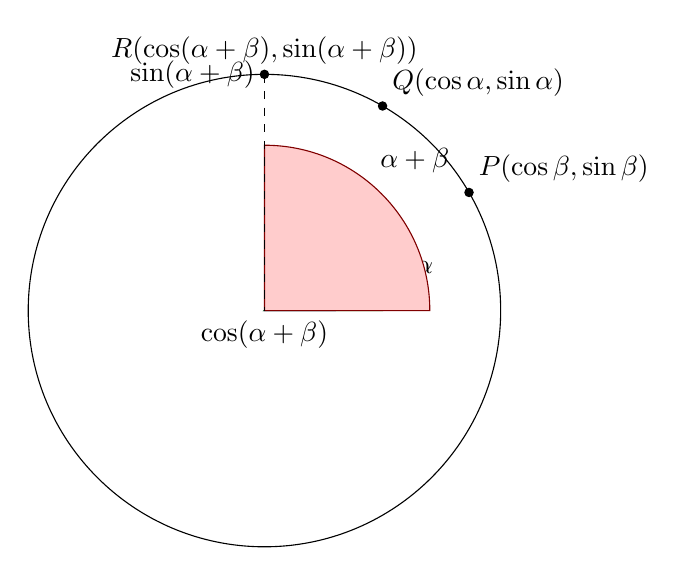
\begin{tikzpicture}[scale=3.0]
% Draw the unit circle
\draw (0,0) circle (1);
% Draw the two angles alpha and beta
\filldraw[fill=green!20,draw=green!50!black] (0,0) -- (0.5,0) arc (0:30:0.5) -- cycle;
\filldraw[fill=blue!20,draw=blue!50!black] (0,0) -- (0.3,0) arc (0:60:0.3) -- cycle;
\node at (15:0.7) {$\alpha$};
\node at (30:0.45) {$\beta$};
% Draw the sum of angles
\filldraw[fill=red!20,draw=red!50!black] (0,0) -- (0.7,0) arc (0:90:0.7) -- cycle;
\node at (45:0.9) {$\alpha + \beta$};
% Draw the corresponding points on the unit circle
\draw[fill=black] (30:1) circle (0.5pt) node[above right] {$P(\cos\beta,\sin\beta)$};
\draw[fill=black] (60:1) circle (0.5pt) node[above right] {$Q(\cos\alpha,\sin\alpha)$};
\draw[fill=black] (90:1) circle (0.5pt) node[above] {$R(\cos(\alpha+\beta),\sin(\alpha+\beta))$};
% Draw the lines for sine and cosine projections
\draw[dashed] (90:1) -- (90:0) node[below] {$\cos(\alpha+\beta)$};
\draw[dashed] (90:1) -- (0,1) node[left] {$\sin(\alpha+\beta)$};
\end{tikzpicture}
\caption{Geometric representation of sum of angles in a unit circle.}
\label{fig:sum_of_angles}
\end{figure}

To gain a better understanding and reinforce these concepts, it is advised to work through some example problems:

\begin{enumerate}
    \item Given that $\sin(\pi/6) = 1/2$ and $\cos(\pi/3) = 1/2$, calculate $\sin(\pi/6 + \pi/3)$.
    \item If $\cos(45^\circ) = \sin(45^\circ) = \frac{\sqrt{2}}{2}$, find the value of $\cos(45^\circ - 45^\circ)$.
    \item Determine $\tan(75^\circ)$ using the tangent sum formula, given that $75^\circ = 45^\circ + 30^\circ$.
\end{enumerate}

The above figure aids in visualizing how the sum of angles is represented within the unit circle, which can further help in understanding how the sum and difference formulas are derived geometrically.

\subsubsection{Practice Problems}
\label{subsubsec:practice_problems_sum_difference}

To ensure a solid grasp of the sum and difference formulas, practice the following problems:

\begin{enumerate}
    \item Evaluate $\sin(75^\circ)$ using the sum formula for sine with $\alpha = 45^\circ$ and $\beta = 30^\circ$.
    \item If $\cos(60^\circ) = \frac{1}{2}$ and $\sin(45^\circ) = \frac{\sqrt{2}}{2}$, find the value of $\cos(60^\circ - 45^\circ)$.
    \item Using the difference formula for tangent, calculate $\tan(15^\circ)$ knowing that $\tan(45^\circ) = 1$ and $\tan(30^\circ) = \frac{\sqrt{3}}{3}$.
    \item Verify the identity $\sin(\alpha + \beta)\sin(\alpha - \beta) = \sin^2(\alpha) - \sin^2(\beta)$ for $\alpha = 60^\circ$ and $\beta = 45^\circ$.
    \item A point P moves in such a way that the angle $\alpha$ it makes with the positive x-axis varies. If $\alpha$ increases at a constant rate of $30^\circ$ per second, express the $x$-coordinate of P, which is $\cos(\alpha)$, as a function of time $t$ in seconds.
\end{enumerate}

These problems combine the use of the sum and difference formulas with some algebraic manipulation and the fundamental trigonometric values for special angles. They serve as a good practice for students to apply these formulas in different contexts, which is a skill that will be beneficial in more advanced studies of mathematics, such as calculus.

% \subsection{Double-Angle and Half-Angle Formulas}
% \label{subsec:double_half_angle_formulas}
% These formulas are useful for integrating powers of sine and cosine functions.

\subsection{Double-Angle and Half-Angle Formulas}
\label{subsec:double_half_angle_formulas}

The double-angle formulas are derived from the sum formulas and provide the trigonometric functions of an angle that is double another. Similarly, the half-angle formulas give the functions of half of a given angle. These are particularly useful in integration and in solving trigonometric equations in calculus.

In conclusion, these formulas are useful for integrating powers of sine and cosine functions.

\subsubsection{Double-Angle Formulas}
\label{subsubsec:double_angle_formulas}
For any angle $\theta$, the double-angle formulas are as follows:

\begin{itemize}
    \item Sine: $\sin(2\theta) = 2\sin(\theta)\cos(\theta)$
    \item Cosine: $\cos(2\theta) = \cos^2(\theta) - \sin^2(\theta) = 2\cos^2(\theta) - 1 = 1 - 2\sin^2(\theta)$
    \item Tangent: $\tan(2\theta) = \frac{2\tan(\theta)}{1 - \tan^2(\theta)}$
\end{itemize}

The cosine double-angle formula has three variants, each useful depending on the context, especially in integration where one expression might be more convenient than the others.

\subsubsection{Half-Angle Formulas}
\label{subsubsec:half_angle_formulas}
The half-angle formulas are derived using the double-angle formulas and the Pythagorean identity. They allow us to express trigonometric functions of $\frac{\theta}{2}$ in terms of $\theta$:

\begin{itemize}
    \item Sine: $\sin\left(\frac{\theta}{2}\right) = \pm\sqrt{\frac{1 - \cos(\theta)}{2}}$
    \item Cosine: $\cos\left(\frac{\theta}{2}\right) = \pm\sqrt{\frac{1 + \cos(\theta)}{2}}$
    \item Tangent: $\tan\left(\frac{\theta}{2}\right) = \pm\sqrt{\frac{1 - \cos(\theta)}{1 + \cos(\theta)}} = \frac{\sin(\theta)}{1 + \cos(\theta)} = \frac{1 - \cos(\theta)}{\sin(\theta)}$
\end{itemize}

The signs for the half-angle formulas depend on the quadrant in which the resulting half-angle lies. These formulas are essential in calculus for simplifying the integration of trigonometric functions and solving trigonometric equations.

\subsubsection{Visualization of Double-Angle and Half-Angle}
\label{subsubsec:visualization_double_half_angle}

To better understand the double-angle and half-angle concepts, it is often helpful to visualize them on the unit circle and through their graphs.

\begin{figure}[H]
\centering
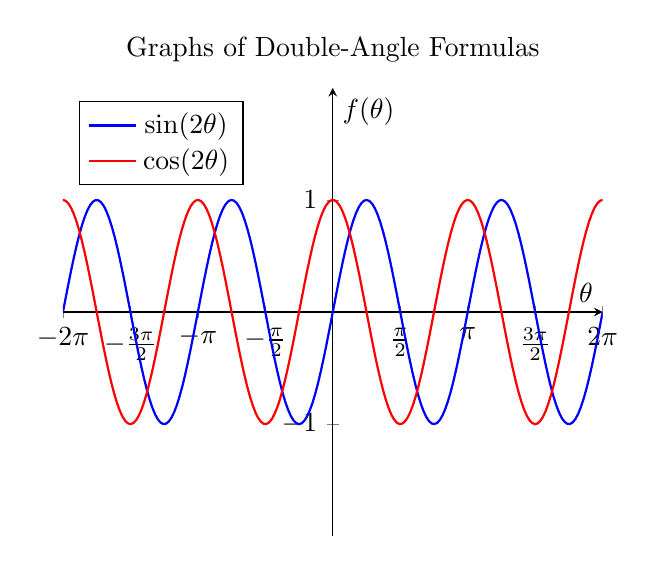
\begin{tikzpicture}
\begin{axis}[
    axis lines = middle,
    xlabel = $\theta$,
    ylabel = {$f(\theta)$},
    legend pos = north west,
    title = {Graphs of Double-Angle Formulas},
    xmin = -2*pi, xmax = 2*pi,
    ymin = -2, ymax = 2,
    xtick = {-6.28318, -4.71239, -3.14159, -1.5708, 0, 1.5708, 3.14159, 4.71239, 6.28318},
    xticklabels = {$-2\pi$, $-\frac{3\pi}{2}$, $-\pi$, $-\frac{\pi}{2}$, $0$, $\frac{\pi}{2}$, $\pi$, $\frac{3\pi}{2}$, $2\pi$},
    ytick = {-1, 1},
    yticklabels = {$-1$, $1$},
    samples = 200,
    domain = -2*pi:2*pi
]

% Add the sine double-angle plot
\addplot[blue, thick] {sin(deg(2*x))};
\addlegendentry{$\sin(2\theta)$}

% Add the cosine double-angle plot
\addplot[red, thick] {cos(deg(2*x))};
\addlegendentry{$\cos(2\theta)$}

\end{axis}
\end{tikzpicture}
\caption{Graphs of $\sin(2\theta)$ and $\cos(2\theta)$.}
\end{figure}

In the graph, we see the effect of doubling the angle on the sine and cosine functions, where the frequency of the waveforms is doubled, reflecting the periodic nature of these functions.

\subsubsection{Problems for Reinforcement}
\label{subsubsec:problems_double_half_angle}
After reviewing the double-angle and half-angle formulas and observing their graphs, tackle the following problems to test your understanding:

\begin{enumerate}
    \item Simplify the expression $\sin(4\theta)$ using the double-angle formula for sine.
    \item Given that $\cos(\theta) = \frac{3}{5}$ and $\theta$ is in the first quadrant, find the exact value of $\cos(2\theta)$.
    \item Use the half-angle formula to determine $\sin\left(\frac{\pi}{8}\right)$, given the cosine and sine of $\frac{\pi}{4}$.
    \item Derive the tangent half-angle formula starting from the sine and cosine half-angle formulas.
    \item Solve the equation $2\sin^2(\theta) - \sin(\theta) - 1 = 0$ for $\theta$ in the interval $[0, 2\pi)$.
\end{enumerate}

\subsubsection{Problems for Reinforcement}
\label{subsubsec:problems_double_half_angle}

\textbf{Problem 1:} Prove that $\cos(4\theta) = 1 - 8\sin^2(\theta) + 8\sin^4(\theta)$ using double-angle formulas.

\textbf{Solution:}
\begin{align*}
\cos(4\theta) &= \cos(2\cdot2\theta) \\
&= 2\cos^2(2\theta) - 1 \quad \text{(Double-angle formula)} \\
&= 2(2\cos^2(\theta) - 1)^2 - 1 \\
&= 2(4\cos^4(\theta) - 4\cos^2(\theta) + 1) - 1 \\
&= 8\cos^4(\theta) - 8\cos^2(\theta) + 1 \\
&= 8(1 - \sin^2(\theta))^2 - 8(1 - \sin^2(\theta)) + 1 \\
&= 1 - 8\sin^2(\theta) + 8\sin^4(\theta).
\end{align*}

\textbf{Problem 2:} If $\tan(\theta) = 3$, find the value of $\tan(2\theta)$.

\textbf{Solution:}
\begin{align*}
\tan(2\theta) &= \frac{2\tan(\theta)}{1 - \tan^2(\theta)} \quad \text{(Tangent double-angle formula)} \\
&= \frac{2\cdot 3}{1 - 3^2} \\
&= \frac{6}{1 - 9} \\
&= -\frac{2}{3}.
\end{align*}

\textbf{Problem 3:} Determine $\cos\left(\frac{\theta}{2}\right)$ if $\sin(\theta) = \frac{1}{2}$ and $\theta$ is in the first quadrant.

\textbf{Solution:}
\begin{align*}
\cos\left(\frac{\theta}{2}\right) &= \pm\sqrt{\frac{1 + \cos(\theta)}{2}} \quad \text{(Cosine half-angle formula)} \\
\text{Since } \sin^2(\theta) + \cos^2(\theta) &= 1, \\
\cos(\theta) &= \sqrt{1 - \sin^2(\theta)} \\
&= \sqrt{1 - \left(\frac{1}{2}\right)^2} \\
&= \sqrt{1 - \frac{1}{4}} \\
&= \sqrt{\frac{3}{4}} \\
&= \frac{\sqrt{3}}{2}. \\
\text{Then, } \cos\left(\frac{\theta}{2}\right) &= \sqrt{\frac{1 + \frac{\sqrt{3}}{2}}{2}} \\
&= \sqrt{\frac{2 + \sqrt{3}}{4}} \\
&= \frac{\sqrt{2 + \sqrt{3}}}{2}.
\end{align*}

\textbf{Problem 4:} Using the double-angle formulas, express $\sin^2(\theta)$ in terms of $\cos(2\theta)$.

\textbf{Solution:}
\begin{align*}
\cos(2\theta) &= 1 - 2\sin^2(\theta) \quad \text{(Cosine double-angle formula)} \\
\sin^2(\theta) &= \frac{1 - \cos(2\theta)}{2}.
\end{align*}

\textbf{Problem 5:} Solve for $\theta$ if $\sin(2\theta) = \sqrt{2}$, assuming $\theta$ is in the second quadrant.

\textbf{Solution:}
\begin{align*}
\sin(2\theta) &= \sqrt{2} \\
2\sin(\theta)\cos(\theta) &= \sqrt{2} \quad \text{(Sine double-angle formula)} \\
\text{Since } \theta &\text{ is in the second quadrant, } \sin(\theta) > 0 \text{ and } \cos(\theta) < 0. \\
\text{Let } \sin(\theta) &= \frac{\sqrt{2}}{2}, \text{ then } \cos(\theta) = -\frac{\sqrt{2}}{2}, \\
\text{and } \theta &= \frac{3\pi}{4} \text{ or } \theta = \frac{5\pi}{4} \text{ to satisfy the quadrant condition.}
\end{align*}

% These problems can be included in the LaTeX document after the discussion of double-angle and half-angle formulas, offering a practical way for students to apply what they've learned. Remember to adjust the problems or solutions according to the level of your students and the specific focus of your course.

% HERE



% Concluding remarks for the chapter
\section*{Conclusion}
\label{sec:trig_conclusion}
This chapter serves as the foundation for understanding the vital role of Trigonometry in calculus. As you progress through your studies, these concepts will become second nature, providing the tools necessary for analyzing and solving a broad range of problems in higher mathematics.

% Ensure that the conclusion is added to the table of contents
\addcontentsline{toc}{section}{Conclusion}

% --- End of Trigonometry Chapter ---




% --- Appendices ---
\clearpage
\addcontentsline{toc}{chapter}{Appendices}
\appendix
\renewcommand{\thechapter}{\Roman{chapter}} % Ensuring chapters are numbered as I, II, III, etc.

%\appendix
\chapter{Basic GitHub Guide}
\section*{A Quick Start to Your GitHub Journey}

Welcome to the fascinating world of GitHub, a platform that has revolutionized the way we collaborate on projects, share code, and build software together. Whether you are a programmer, a writer, or a mathematician, GitHub provides a set of powerful tools to help you collaborate with others, manage your projects, and contribute to the vast world of open-source software. In this guide, we will walk you through the foundational steps to get started with GitHub, helping you to navigate, contribute, and make the most out of this incredible platform.

\subsection*{Creating Your GitHub Account}

The first step to joining the GitHub community is to create an account. Here’s how you can do it:

\begin{enumerate}
    \item Visit the \href{https://github.com/}{GitHub website}.
    \item Click on the “Sign up” button.
    \item Fill in the required information, including your username, email address, and password.
    \item Verify your account and complete the sign-up process.
\end{enumerate}

Once you have created your account, take a moment to explore your new GitHub dashboard. Here, you will find a variety of tools and features that will help you manage your projects, collaborate with others, and discover new and interesting repositories.

\subsection*{Creating Your First Repository}

A repository (or “repo”) is a digital directory where you can store your project files. Here’s how you can create your first repository:

\begin{enumerate}
    \item From your GitHub dashboard, click on the “New” button to create a new repository.
    \item Give your repository a name and provide a brief description.
    \item Initialize this repository with a README file. (This is an optional step, but it’s a good practice to include a README file in every repository to explain what your project is about.)
    \item Click “Create repository.”
\end{enumerate}

Congratulations! You have just created your first GitHub repository. You can now start adding files, collaborating with others, and managing your project right from GitHub.

\subsection*{Making Changes and Commits}

GitHub uses Git, a version control system, to keep track of changes made to your project. Here’s a quick guide on how to make changes and commits:

\begin{enumerate}
    \item Navigate to your repository on GitHub.
    \item Find the file you want to edit, and click on it.
    \item Click the pencil icon to start editing.
    \item Make your changes and then scroll down to the “Commit changes” section.
    \item Provide a commit message that explains the changes you made.
    \item Choose whether you want to commit directly to the main branch or create a new branch for your changes.
    \item Click “Commit changes.”
\end{enumerate}

Your changes are now saved, and a new commit is created. Every commit has a unique ID, making it easy to track changes, revert to previous versions, and collaborate with others.

\subsection*{Collaborating with Others}

One of the biggest strengths of GitHub is its collaborative nature. Here are some ways you can collaborate with others:

\begin{itemize}
    \item \textbf{Forking:} You can fork a repository, create your own copy, make changes, and then propose those changes back to the original project.
    \item \textbf{Issues:} Use issues to report bugs, request new features, or start a discussion with the community.
    \item \textbf{Pull Requests:} Propose changes to a project by creating a pull request. This allows others to review your changes, discuss them, and eventually merge them into the project.
\end{itemize}

\subsection*{Conclusion: Embarking on Your GitHub Adventure}

Now that you have a basic understanding of GitHub and how it works, you are ready to embark on your GitHub adventure. Explore repositories, contribute to open-source projects, collaborate with others, and build amazing things together. Remember, the GitHub community is vast and supportive, and there is a wealth of knowledge and resources available to help you along the way. Happy coding!

\chapter{Basic \LaTeX\ Guide}
\section*{A Quick Start to Your \LaTeX\ Journey}

Welcome to the immersive world of \LaTeX, a typesetting system widely used for creating scientific and professional documents due to its powerful handling of formulas and bibliographies. This guide is designed to offer you the foundational steps to grasp the basics of \LaTeX, enabling you to craft documents of high typographic quality akin to this book.

\subsection*{Setting Up Your \LaTeX\ Environment}

Before you can start creating documents with \LaTeX, you need to set up a working \LaTeX\ environment on your computer. Here's how you can do it:

\begin{enumerate}
    \item Download and install a \TeX\ distribution, which includes \LaTeX. For Windows, MiKTeX is a popular choice, while Mac users might prefer MacTeX, and TeX Live is widely used on Linux.
    \item Install a \LaTeX\ editor. Some popular options include TeXShop (for Mac), TeXworks (cross-platform), and Overleaf (an online \LaTeX\ editor).
    \item Ensure that your \TeX\ distribution and \LaTeX\ editor are properly configured and integrated.
\end{enumerate}

\subsection*{Creating Your First \LaTeX\ Document}

Once your \LaTeX\ environment is set up, you are ready to create your first \LaTeX\ document. Follow these steps:

\begin{enumerate}
    \item Open your \LaTeX\ editor and create a new document.
    \item Insert the following code to set up a basic \LaTeX\ document:

\begin{verbatim}
\documentclass{article}
\begin{document}
Hello, \LaTeX\ world!
\end{document}
\end{verbatim}

    \item Save your document with a .tex file extension.
    \item Compile your document using your \LaTeX\ editor. This process converts your .tex file into a PDF document.
    \item View the output PDF and admire your first \LaTeX\ creation.
\end{enumerate}

\subsection*{Understanding \LaTeX\ Commands and Environments}

\LaTeX\ documents are created using a series of commands and environments. Commands typically start with a backslash \textbackslash\ and are used to format text, insert special characters, or execute functions. Environments are used to define specific sections of your document that require special formatting.

\begin{itemize}
    \item \textbf{Commands:} For example, \textbackslash\textit\{italics\} will render the word "italics" in italic font.
    \item \textbf{Environments:} To create a bulleted list, you would use the \textit{itemize} environment:

\begin{verbatim}
\begin{itemize}
    \item First item
    \item Second item
\end{itemize}
\end{verbatim}
\end{itemize}

\subsection*{Adding Structure to Your Document}

\LaTeX\ makes it easy to structure your documents with sections, subsections, and chapters. Here’s how you can add structure:

\begin{verbatim}
\section{Introduction}
This is the introduction of your document.
\subsection{Background}
This subsection provides background information.
\subsubsection{Details}
This is a subsubsection for more detailed information.
\end{verbatim}

\subsection*{Including Mathematical Formulas}

\LaTeX\ excels at typesetting mathematical formulas. Use the \textit{equation} environment or the \textdollar\ sign for inline formulas. For example:

\begin{verbatim}
The quadratic formula is \( x = \frac{-b \pm \sqrt{b^2 - 4ac}}{2a} \).
\end{verbatim}

\subsection*{Adding Images and Tables}

You can also include images and tables in your \LaTeX\ documents:

\begin{itemize}
    \item \textbf{Images:} Use the \textit{graphicx} package and the \textit{includegraphics} command.
    \item \textbf{Tables:} Use the \textit{tabular} environment to create tables.
\end{itemize}

\subsection*{Compiling Your Document}

\LaTeX\ documents need to be compiled to produce a PDF. This can be done through your \LaTeX\ editor. If your document includes bibliographies or cross-references, you may need to compile multiple times.

\subsection*{Conclusion: Embracing the Power of \LaTeX}

Congratulations! You have taken your first steps into the world of \LaTeX. With practice, you will discover that \LaTeX\ is a powerful tool for creating professional-quality documents, from simple articles to complex books. Embrace the learning curve, explore the vast array of packages available, and join the community of \LaTeX\ users who are ready to help you on your journey. Happy typesetting!

% --- Bibliography ---
\addcontentsline{toc}{chapter}{Bibliography}
\bibliographystyle{alpha}
\bibliography{references} % Assuming you have a references.bib file

% --- Index ---
% \addcontentsline{toc}{chapter}{Index}
% \printindex

\end{document}
